\documentclass[uplatex,dvipdfmx,openany,oneside,report]{bxjsbook}
\usepackage{okumacro,plext}
\usepackage{natbib}
\usepackage{url}
\usepackage{chapterbib}
\usepackage{txfonts}
\usepackage[utf8]{inputenc}
\usepackage[T1]{fontenc}
\usepackage{otf}
\usepackage{tabularx}
%\usepackage{my_resume}
%\usepackage{graphicx,wrapfig}
%\usepackage[greek,english]{babel}
%\usepackage{teubner}
%\usepackage[dvipdfm,bookmarkstype=toc=true,pdfauthor={江口聡, EGUCHI Satoshi}, pdftitle={}, pdfsubject={},pdfkeywords={},bookmarks=false, bookmarksopen=false,colorlinks=true,urlcolor=blue,linkcolor=black,citecolor=black,linktocpage=true]{hyperref}
%  \AtBeginDvi{\special{pdf:tounicode EUC-UCS2}}% platex-utf8 でも OK
\author{江口聡}
\title{京女生のためのミニマム社会思想入門}
\if0 %----------------------------------------------------------------
\fi  %----------------------------------------------------------------

\newcommand\mybook{}



\begin{document}


\maketitle{}
\frontmatter

\tableofcontents{}
\ifx\mybook\undefined
\documentclass[autodetect-engine,dvipdfmx-if-dvi,ja=standard]{bxjsarticle} \usepackage{mystyle}
\author{江口聡}
%\date{}
\title{なぜ社会思想を学ぶか}
\if0 %----------------------------------------------------------------

\fi  %----------------------------------------------------------------
\begin{document}
\maketitle

\else
\chapter*{はじめに:なぜ社会思想を学ぶか}
\fi
\addcontentsline{toc}{chapter}{はじめに:なぜ社会思想を学ぶか}

歴史や社会思想についての知識は、大学生・市民としての基礎教養である。大学4年間での学習・研究のため、このテキスト程度のことは理解しておいてほしい。

若い人々には気づきにくいことだが、人間の社会は大きく変化してきた。そしてこれからも社会は変わる!その変化に対応していくため、そして変化をよい方向にもっていくためにも、社会の変化の背景にある思想とその変化についてある程度の知識をもっておきたい。方針としては、断片でもいいのでなるべく思想家たちの生の言葉を味わって欲しいと考えている。




% 公務員試験、教職、入社試験 → このテキスト程度で「人文」教養の6、7割とれることを目指す。

% 授業ではだいたい古代ギリシアから20世紀初頭までの西洋思想を扱う。


\section*{問題意識}


人類の歴史のある時点から、人間は、自分たち人間と社会はどんなものであるか、どうあるべきか、社会の成り立ちはどんなものであるか、どうあるべきか、といったことを考えはじめる。社会状況が思想を生み、誰かの思想が社会状況を変革する。





次のような問題意識をもって半期学んでほしい。

\begin{itemize}
\item 「自由」「平等」「正義」「人権」「人民主権」「民主主義」「市民」「選挙権」「福祉国家」「生命尊重」「市民的不服従」といったさまざまな概念とその由来。
\item 国家とはなにか?それはなんのためにあるのか?法はなぜ必要か?どのような法がよい法か?

\item 社会のルールはどのようにして決まるのか? どのようにして決める\kenten{べき}か。

\item 社会的動物としての人間とはどのような存在だと考えらてきたか?

\item 現在は当然の権利と考えられているが以前はそうでなかったものにはどのようなものがあるか?

\item 国家どうしの関係(国際関係)はどうあるべきだと理解されていたか?現在はどう考えられているか?

\item 新しい発想や考え方が出てきたときに、\kenten{それまでに存在しなかったもの}を考えてみよう。

\end{itemize}






\section*{勉強ティプス}

\begin{itemize}

\item 年代はだいたいで覚える。細かいのは無理。〜世紀初頭、前半、なかば、後半、末、程度のおぼえかたでよい。

\item \emph{高校世界史の教科書と資料集}を手元に置いておく。年表を自分で作ってみるのもよい。高校で世界史を十分履修していない人は、まず中学校の「歴史」を確認しておこう。
\item 歴史の本はどんどん読むこと。高校で勉強されられた政治史中心の歴史よりは、もの(たとえば胡椒や砂糖)の歴史、文化(恋愛や結婚制度、帳簿、武器・戦争技術など)の歴史などがおもしろいだろう。
\item 人の名前は覚えにくい。肖像画や写真といっしょにすると覚えやすい。アルファベットでの綴り字も一応確認しておくと恥ずかしい読み間違いが減る(おぼえる必要はない)。人名、出来事等は、さっさとWikipediaなどで確認する癖をつけたい。Wikipediaもどんどん使う。
\item 河出書房新社の「ふくろうの本」シリーズ、新潮社の「とんぼの本」シリーズのような図版を中心にしたヴィジュアル本が読みやすいし印象に残りやすい。\emph{岩波ジュニア新書}も大学1回生で読むのにぴったりなので図書館を利用する。『砂糖の歴史』『フランス革命』など名著。

\item NHKの『映像の世紀』に代表される歴史と科学のテレビ番組もどんどん見よう。

\item 大学での勉強の仕方、ノートの取り方など研究すること。

\end{itemize}





\section*{おすすめ本}
\begin{itemize}
\item 水田洋、『社会思想小史』、ミネルヴァ書房、2006。
\item ミシェリン・イシェイ、『人権の歴史』、明石書店、2008。
\item リン・ハント、『人権を創造する』、岩波書店、2011。
\item スティーブン・ピンカー、『暴力の人類史』、2015。
\item ウィリアム・H・マクニール (2007) 『疫病と世界史』、中公文庫
\item ウィリアム・H・マクニール (2014) 『戦争の世界史』、中公文庫
\item   ウィリアム・H・マクニール (2008) 『世界史』、中公文庫
\item ジャレド・ダイアモンド (2012) 『銃・病原菌・鉄』、草思社文庫
\item ジャレド・ダイアモンド (2012) 『文明崩壊』、草思社文庫
\item デヴィッド・クリスチャン (2015) 『ビッグヒストリー入門』、WAVE出版
\item ユヴァル・ノア・ハラリ (2016) 『ホモ・サピエンス全史』、河出書房新社
\item 川北稔 (1996) 『砂糖の世界史』、岩波ジュニア新書

  
  
\end{itemize}


\nocite{Pinker11:angel}
\nocite{hunt07:_inven_human_right}
\nocite{水田洋06:社会思想小史}
\nocite{ishay04:_histor_human_right}





\ifx\mybook\undefined
%\addcontentsline{toc}{chapter}{\bibname}
\bibliographystyle{jecon}
%\bibliography{bib}


\end{document} %----------------------------------------------------------------
\fi




\nocite{納富信留06:ソフィスト}


%%% Local Variables:
%%% mode: japanese-latex
%%% TeX-master: t
%%% coding: utf-8
%%% End:

\mainmatter
\documentclass[uplatex,dvipdfmx]{jsarticle} \usepackage{mystyle}%\author{} %date{}
\title{原始国家〜古代ギリシア}
\if0 %----------------------------------------------------------------

\fi  %----------------------------------------------------------------
\begin{document}
\maketitle

% \chapter{古代ギリシア}\fi



\section{古代ギリシアのポリス社会}

\subsection{ポリス}

\begin{itemize}
\item ギリシア。紀元前8世紀ごろ、人々が集住して都市「\emph{ポリス}」ができる。
\item 古代ギリシアの\emph{ポリス}国家。城壁で囲まれた都市が一つの国家。
\item 「国家」とは? 現代的に考えると、(1) 土地、(2)人民、(3)主権をもっている人の集団が国家。「主権」とは他の国から独立に意思決定をおこなうこと。それ以上の決定組織がない。国民から税金を集めたり、戦争したりする決定力をもっているのが国。
\item 各ポリスによって制度・法律はさまざま。\emph{王政}の国(王が最終的な決定権をもつ)、\emph{共和制}(王が存在せず、国家元首を直接・間接に選出したり、複数の代表者を置いたりする)・\emph{民主制}(共和制のなかでも、国民全体の意志にもとづく政治をおこなう)の国など。
アテネのライバル国家のスパルタは王政(貴族制)。

\end{itemize}

\subsection{アテネの民主制}
\begin{itemize}
\item アテネの民主制が民主主義の原点として有名で、世界史的に重要とされている。
\item 奴隷と戦争の重要性。土地と奴隷を確保するための戦争が頻繁にある。騎馬を利用する貴族による戦争から、次第に富裕な平民が武具を用意して重装歩兵として活躍するようになる。平民が戦争参加の見返りに参政権を主張し貴族と対立。
\item 紀元前7世紀のドラコン法による「法の支配」(法治主義)(⇔ 人の支配(人治主義))。紀元前6世紀初頭ソロンの改革。血統ではなく財産額による参政権(財産政治)。
\item 非合法な独裁者である僭主(tyranny)の登場。法には反するが、平民の支持があった。→ 僭主政治の崩壊、僭主の出現を予防する陶片追放(オストラシズム)制度の採用。
\item 紀元前5世紀はアテネの黄金時代。
\item 人口20万程度の(当時の)大都市。奴隷もいた(20万人中の8万人ぐらいか)。
\item 「市民」(国民)とされるのは財産をもった成人男性。戦争になれば自分で装備して出兵する。中上流家庭の女性は家の外に出なかった。
\item 621B.C. ドラコン法(慣習法を成文化)。→ 僭主(独裁者)の登場 → 陶片追放(オストラシズム)制度で潜主の再登場を避けようとする。
\item ペルシア戦争(500 B.C. -- 449 B.C.)。
\item ペリクレス時代(443 B.C. -- 429 B.C.)。ペリクレスは民主制を称えた演説でも有名。直接民主制、官職は抽選。参政権は自由市民男子のみ。裁判も選出された裁判員の多数決。
\item アテネとスパルタとのペロポネソス戦争(431B.C. -- 404. B.C.)。
\item 扇動政治家(デマゴーク)が出現することもあった。 → 「デマ」の語源。
\item 市民の没落。傭兵の流行。
\item マケドニアが勢力を伸ばす。アレクサンドロス大王(336 B. C. -- 323 B.C.)がエジプト征服、ペルシアを滅ぼし、東方遠征。
\item アレクサンドロスの死後、アンティゴノス朝マケドニア、セレウコス朝シリア、プトレマイオス朝エジプトに分裂。アレクサンドロスからプトレマイオス朝エジプトの滅亡までが\emph{ヘレニズム時代}。
\end{itemize}


\section{ソフィストたち}

\begin{itemize}
\item ポリス社会では「弁論」が重要。投票で政治を決め、裁判も投票制なので弁論の技術が大事になる。
 → 弁論を教える職業的教師\emph{ソフィスト}(「知者」の意味)の登場。
\item プロタゴラスの「人間は万物の尺度」という言葉の代表されるように、\emph{相対主義}的な考え方を好む。
\item \emph{ノモス}(法、道徳)と\emph{ピュシス}(自然)を区別する。法や道徳などの社会のルール(ノモス)は人間が作りだしたものにすぎない。だから我々は弱肉強食の自然のルール(ピュシス)にしたがって、ズルできるときはするべきだ、といった主張がなされる。
\item → \emph{相対主義}。善悪、正・不正は社会の決め事にすぎず、社会によって違う。すべての社会に共通の「本当に正しいこと」などは存在せず、実は力の対立があるだけだけである。我々はよく生きようとすれば、知恵と力をつかって他人を支配しなければならない。

\end{itemize}




\section{ソクラテス}


\begin{itemize}
\item 元祖「哲学者」
\item 友人がデルフォイの神殿で「一番賢いのはソクラテスだ」という神託を受ける。「自分は賢い」と公言している人々(ソフィストや政治家たち)は本当に賢いのか?
\item 「汝自身を知れ」「ただ生きることではなくよく生きることが重要だ」「吟味されない生は生きるに値しない」などの言葉で知られる。
\item 知への愛 → 哲学 → 19世紀ごろまで学問はなんでも「哲学」。
\item ソフィストや政治家たちは、たとえば「善とは何か」「正義とは何か」を本当に知っているのか?

\item 議論・談論の重要性。
\end{itemize}

  \begin{quote}
    人間にとっては、徳その他のことについて、毎日談論するという、このことが、まさに最大の善きことなのであって、わたしがそれらについて、問答しながら、自分と他人を吟味しているのを、諸君は聞かれているわけであるが、これに反して、吟味のない生活は、人間の生きる生活ではないと、こう言っても、わたしがこう言うのを、諸君はなおさら信じないであろう。しかしそのことは、まさにわたしの言うとおりなのだ、諸君。ただそれを信じさせることが、容易ではないのです。(38a)
  \end{quote}
  \begin{itemize}

\item 問答法(対話法)。 → ソクラテス的方法 (Socratic method)。演説や教授ではなく、対話・問答によって真理を発見する。(しかしたいてい喧嘩別れ。はっきりした答はなかなか出てこない。)
\end{itemize}

  \begin{quote}
     わたしとは、どんな人間であるかといえば、もしわたしの言っていることに何か間違いでもあれば、こころよく反駁を受けるし、他方また、ひとの言っていることに何か本当でない点があれば、よろこんで反駁するような、とはいっても、反駁を受けることが、反駁することに比べて、少しも不愉快にならないような、そういう人間なのです。なぜなら、反駁を受けることの方が、より大きな善であるとわたしは考えているからです。(『ゴルギアス』 458A )
  \end{quote}
\begin{itemize}

\item 「無知の知」。知恵のある者(ソフィスト)ではなく、知恵を愛する者、知恵を求める者(phil 愛 + sophia 知恵 → philosophoi 哲学者\footnote{明治期に西周は当初philosophyを、哲を求める学問として希哲学と訳した。})。以降学者は自然科学者も含めてすべて「哲学者」を自称することになる。博士号 Ph.~D.は Philosophiae Doctor 「哲学博士」の略号。

\item 子どもに、その子どもにとって善いものを与えることと、子どもが欲するものを与えることはまったく違う。 → 「善い」ことは「本人が欲すること」とは違う。

\item 自由とは欲望のままに行動することではない。独裁者になって他人を殺すより、正しく生きて独裁者に殺される方が幸福でありよく生きている。

\item 健康、強さ、美しさ、富などは一般に有益であるが、時に害を与えることがある。それを\kenten{正しく} 使用するときに有益。節制、正義、勇気、理解力、寛大さなども知性がともなわなければ有害なことがある。

\item   → したがって徳は知。徳(aret\={e}, virtue)の基本の意味は「すぐれてある」こと、卓越性、能力。悪徳は無知による。

\item ソクラテスは新しい神を祭り若者に悪影響を与えるとして裁判にかけられ、死刑を宣告される。友人たちが脱獄をすすめるが、断わり毒を飲んで死ぬ。

\end{itemize}

\section{プラトン}

\begin{itemize}
\item ソクラテスの弟子の一人。ソクラテスの言行を書き残す(他にも政治家クセノポンや喜劇作家アリストパネスなどもソクラテスの言行を書き残している)。『ソクラテスの弁明』『クリトン』『ゴルギアス』など。
\item 学園アカデメイアを創設する。
\item 『国家』では自身の立場で政治を探究。正義とそれを実現する理想的な国家のあり方を考える。
\item 民主制(デモクラティア)を強烈に批判。ソクラテスを刑死させたように、(劣った)大衆の判断は当てにならない。
\item 人間には生まれつきの素質の上下がある。
\item 人間の魂が欲望と意志と理性に分けられるように、国家も生産者と防衛者と統治者に分けられる。
\item 統治者と防衛者は国家のために私的な欲望を捨てなければならない。→ 財産は持たない → 子どもは家族ではなく国家が養育する。
\item 統治者は子どものころから特別な教育を受ける必要がある。
\item 哲人王が統治する王政がベストの政体。民主制は必然的に腐敗する。
\end{itemize}


\section{アリストテレス}
\begin{itemize}
\item プラトンの弟子。アカデメイアで学んだのちに、学園リュケイオンを設立。散歩しながら議論したので逍遥学派と呼ばれる。
\item 現代で言えば文学、天文学、物理学、生物学など広範囲の学問の書物を残し、「万学の祖」と呼ばれる。→ アラビア語に翻訳され、中世にふたたびヨーロッパにもたらされる。近世のはじめまで自然科学についての権威とされていた。
\item 「人間は社会的動物である。」
\item 幸福=よく生きる≠単に楽しく暮らす。
\item よく生きる=人間の能力(徳)の発揮 = 自己実現。
\item 徳(アレテー)=卓越性。
\item 倫理的徳と知的徳。倫理的徳については「中庸」がベスト。勇気という徳は、臆病と蛮勇の中間、気前のよさという徳はケチと浪費の中間。
\item 正義(ディカイオシュネー)。正義にはいくつか意味がある。応報的正義。善には善を、悪には悪を与える。分配的正義 = 名誉や財産の正しく平等な分配。匡正的正義 = 平等な関係が不当に侵されたときに、悪に罰を加え、善に報奨を与える正義。
\item 友愛(ピリア)。ポリスは他者を承認し尊重しあう共同体(コイノニア)。

\item 国家体制
  \begin{itemize}
  \item × 単なる多数決による民主制。貧しいものの利益だけが追求される。
  \item × 僭主独裁制。少数のものの利益だけが追求される。
  \item 王政。王が法にしたがって市民全体の利益を追求する。
  \item 優秀者支配。エリートたちが市民全体の利益を追求。
  \item 国政(ポリーテイアー)。よき指導者のもとで市民全体の利益を追求する民主制(共和制)。
  \end{itemize}
\end{itemize}


\fi
\ifx\mybook\undefined
\bibliographystyle{eguchi}
\bibliography{bib}


\end{document} %----------------------------------------------------------------

\fi





%%% Local Variables:
%%% mode: japanese-latex
%%% TeX-master: t
%%% coding: utf-8
%%% End:

\ifx\mybook\undefined
\documentclass[uplatex,dvipdfmx]{jsarticle} \usepackage{mystyle}%\author{} %date{}
\title{}
\if0 %----------------------------------------------------------------

\fi  %----------------------------------------------------------------
\begin{document}
\maketitle


\else\chapter{ユダヤ・キリスト教・イスラーム}

\fi
\section{ユダヤ教}


\subsection{ユダヤ民族の宗教}


\begin{itemize}
\item 当時の他の多くの地域では\emph{多神教}が普通。ユダヤ教の特異さ = \emph{一神教}。
  神は一人だけ。人格をもった神(人格神)。
\item 律法=神との契約。民族の祖アブラハムが神と最初の契約を結ぶ。
\item モーセに戒律(十戒)が与えられる。
\item 預言者(神の言葉を聞いた者)と呼ばれる宗教・政治的リーダー。
\item 戒律の重視。→ 戒律を守るのが「ユダヤ人」。選民思想。
\item 旧約聖書\footnote{ただし「旧約」「新約」という呼び方はキリスト教からのもの。}は歴史書であると同時に神とユダヤ民族の契約の書。

\end{itemize}

\section{イエス}


\begin{itemize}

\item イエス\footnote{学術的な文脈では、「キリスト」とは呼ばないことが多い。}の革新的思想。
「山上の垂訓」は必ず読んでおくこと。
\item 黄金律(the Golden Rule)「人にしてもらいたいと思うことは何でも、あなたがたも人にしなさい。」(マタイ12:7)
\item 新約聖書。イエスとその弟子たちの言行録と手紙。イエス自身が新しい宗教を確立したわけではない。
パウロ中心に教義を完成。イエスによって神との契約が成就されたと解釈。
\item 「神の王国」という思想。神が王として世界を支配する。
\item パウロ。「イエスはキリストであり、人類の罪を贖った。」→ 「キリスト教」の成立。原罪、贖罪、復活、三位一体などの教義。
\item 隣人愛。
\item 性的禁欲。
\item 「神の国」という思想。神が王として世界を支配する。
\item ローマ帝国で迫害される(当時のローマは多神教)。殉教。
\item → 4世紀はじめに公認 → 後半に国教に。

\end{itemize}


\section{中世キリスト教}

\begin{itemize}
\item 古代ギリシア思想と融合。
\item 4-5世紀。アウグスティヌス。「原罪」の強調。
\item 理性と信仰。対立?  → ずっと問題。信仰の方が上位にあるという考え方が主流。
\item 禁欲的。
\item 西洋国家と宗教。ローマ教皇が皇帝・国王を任命。
\item ローマ教皇の権威は12世紀ごろ頂点。十字軍派遣。
\end{itemize}





\section{イスラーム}


\begin{itemize}

\item ムハンマドが最後の預言者。(神ではない。信仰の対象はあくまで唯一神。)
\item クルアーン(コーラン)は神からの啓示。
\item 最近は「イスラム教」とは呼ばない。イスラームは単なる宗教ではなく、社会制度・政治経済まで含めた広い概念。
\item \emph{六信}。アッラー、啓典、預言者、天使、最後の審判、天命。

\item 唯一神信仰。ユダヤ教やキリスト教と共通。絶対帰依。
\item モーセやイエスも預言者の一人。(イエスは預言者であって神ではない)
\item 五行。\ruby{信仰告白}{シャハーダ}、\ruby{礼拝}{サラート}、\ruby{喜捨}{ザカート}、\ruby{断食}{サウム}、\ruby{巡礼}{ハッジ}。
\item ウンマ=ムスリムの信仰共同体。
\item 飲酒禁止。豚肉禁忌。異教徒が殺した動物も×。利子をとることの禁止。
\item 政教一致。
\item 結婚に際しての明示的契約。一夫多妻を許容。チャドルの使用。左手は不浄。
\item 商業の肯定。(キリスト教は否定的)
\item カリフの座をめぐっての争いで分裂。世界史の教科書でシーア派の由来など確認しておくこと。
\item 8世紀、イスラーム帝国。学術も発展。
\end{itemize}



\section{ローマ帝国とキリスト教}

\begin{itemize}
\item キリスト教はローマ帝国で4世紀はじめに公認。4世紀後半には国教化。
\item 4世紀後半のゲルマン民族の大移動 → ローマ帝国の領土縮小。
\item 4世紀後半、西ローマ帝国滅亡。ゲルマン民族のフランク王国成立 → キリスト教に改宗。
\item 9世紀初頭、カール大帝が西ローマ帝国皇帝に戴冠。
\end{itemize}







\section{封建社会}

\begin{itemize}
\item ローマの恩貸制度。家臣の奉仕を義務に、土地の使用権を貸し与える。
\item ゲルマン国家の従士制。貴族に仕えることによって衣食や武器を給与される。
\item → 中世封建領主。諸侯や騎士は独立した領主として土地を支配・経営。契約によって他の領主に仕える。
\item 諸侯・騎士どうしの関係。家臣は主君に戦争その他での忠節を近い、主君は家臣に土地を与える。
\item 土地には農奴(不自由農民、賦役や貢租を求められる)が付属する。
\item 教会権力と世俗権力の両立。世俗的権力を神の名によって正当化・権威づけ。皇帝や国王は異教徒の侵入からキリスト教世界を防衛する。
\item 次第に世俗権力と教会権力は対立するようになる。
\item 11世紀からの十字軍 → 世俗(国王)権力の増大
\item → 中世封建社会は次第に動揺。
\end{itemize}



\section{キリスト教の国家論}

\subsection{アウグスティヌス}

\begin{itemize}
\item ヒッポのアウグスティヌス(354-430)。キリスト教の教義の土台を据えた「教父」の一人。『神の国』など。
\item 人間はアダムとイブから遺伝している「原罪」を背負った罪人。イエス・キリストが罪を許し\ruby{贖}{あがな}う。
\item 『神の国』では「地の国」と「神の国」との対立が描かれる。神の国は人類の歴史が終るときに成就する。世俗国家(地の国)は神の国の理念に反してはならず、教会を見習うべき。
\item → キリスト教の権威が世俗の権威(皇帝権など)を正当化するという思想。

\end{itemize}


\subsection{トマス・アクィナス}
\begin{itemize}
\item トマス・アクィナス(1225-74)。
\item 自然法思想。ローマ時代から存在していた考え方で、人間が定めた法(実定法)に先行して、自然の法が存在しているという思想。
\item トマスは神の永遠の法が人間に示されたときに自然法と呼ばれると考える。人間が定める実定法は、神の永遠の法にしたがって共通善を目指さねばならない。
\end{itemize}



\if0

\section{旧約・新訳聖書から}



\subsection*{『出エジプト記』第20章から(モーセの十戒)}

神はこれらすべての言葉を告げられた。「わたしは主、あなたの神、あなたをエジプトの国、奴隷の家から導き出した神である。あなたには、わたしをおいてほかに神があってはならない。あなたはいかなる像も造ってはならない。上は天にあり、下は地にあり、また地の下の水の中にある、いかなるものの形も造ってはならない。あなたはそれらに向かってひれ伏したり、それらに仕えたりしてはならない。わたしは主、あなたの神。わたしは熱情の神である。わたしを否む者には、父祖の罪を子孫に三代、四代までも問うが、わたしを愛し、わたしの戒めを守る者には、幾千代にも及ぶ慈しみを与える。あなたの神、主の名をみだりに唱えてはならない。みだりにその名を唱える者を主は罰せずにはおかれない。安息日を心に留め、これを聖別せよ。六日の間働いて、何であれあなたの仕事をし、七日目は、あなたの神、主の安息日であるから、いかなる仕事もしてはならない。あなたも、息子も、娘も、男女の奴隷も、家畜も、あなたの町の門の中に寄留する人々も同様である。六日の間に主は天と地と海とそこにあるすべてのものを造り、七日目に休まれたから、主は安息日を祝福して聖別されたのである。あなたの父母を敬え。そうすればあなたは、あなたの神、主が与えられる土地に長く生きることができる。殺してはならない。姦淫してはならない。盗んではならない。隣人に関して偽証してはならない。隣人の家を欲してはならない。隣人の妻、男女の奴隷、牛、ろばなど隣人のものを一切欲してはならない。」



\subsection*{マタイによる福音書 5章から}

イエスはこの群衆を見て、山に登られた。腰を下ろされると、弟子たちが近くに寄って来た。
そこで、イエスは口を開き、教えられた。


\subsubsection*{姦淫してはならない}



「あなたがたも聞いているとおり、『姦淫するな』と命じられている。しかし、わたしは言っておく。みだらな思いで他人の妻を見る者はだれでも、既に心の中でその女を犯したのである。もし、右の目があなたをつまずかせるなら、えぐり出して捨ててしまいなさい。体の一部がなくなっても、全身が地獄に投げ込まれない方がましである。もし、右の手があなたをつまずかせるなら、切り取って捨ててしまいなさい。体の一部がなくなっても、全身が地獄に落ちない方がましである。」

\subsubsection*{復讐してはならない}

「あなたがたも聞いているとおり、『目には目を、歯には歯を』と命じられている。しかし、わたしは言っておく。悪人に手向かってはならない。だれかがあなたの右の頬を打つなら、左の頬をも向けなさい。あなたを訴えて下着を取ろうとする者には、上着をも取らせなさい。 だれかが、一ミリオン行くように強いるなら、一緒に二ミリオン行きなさい。求める者には与えなさい。あなたから借りようとする者に、背を向けてはならない。」

\subsubsection*{敵を愛しなさい}

「あなたがたも聞いているとおり、『隣人を愛し、敵を憎め』と命じられている。しかし、わたしは言っておく。敵を愛し、自分を迫害する者のために祈りなさい。あなたがたの天の父の子となるためである。父は悪人にも善人にも太陽を昇らせ、正しい者にも正しくない者にも雨を降らせてくださるからである。自分を愛してくれる人を愛したところで、あなたがたにどんな報いがあろうか。徴税人でも、同じことをしているではないか。自分の兄弟にだけ挨拶したところで、どんな優れたことをしたことになろうか。異邦人でさえ、同じことをしているではないか。だから、あなたがたの天の父が完全であられるように、あなたがたも完全な者となりなさい。」


\subsubsection*{施しをするときには}

「見てもらおうとして、人の前で善行をしないように注意しなさい。さもないと、あなたがたの天の父のもとで報いをいただけないことになる。だから、あなたは施しをするときには、偽善者たちが人からほめられようと会堂や街角でするように、自分の前でラッパを吹き鳴らしてはならない。はっきりあなたがたに言っておく。彼らは既に報いを受けている。施しをするときは、右の手のすることを左の手に知らせてはならない。あなたの施しを人目につかせないためである。そうすれば、隠れたことを見ておられる父が、あなたに報いてくださる。」


\subsubsection*{神と富}



「だれも、二人の主人に仕えることはできない。一方を憎んで他方を愛するか、一方に親しんで他方を軽んじるか、どちらかである。あなたがたは、神と富とに仕えることはできない。」

\subsubsection*{思い悩むな}

「だから、言っておく。自分の命のことで何を食べようか何を飲もうかと、また自分の体のことで何を着ようかと思い悩むな。命は食べ物よりも大切であり、体は衣服よりも大切ではないか。空の鳥をよく見なさい。種も蒔かず、刈り入れもせず、倉に納めもしない。だが、あなたがたの天の父は鳥を養ってくださる。あなたがたは、鳥よりも価値あるものではないか。あなたがたのうちだれが、思い悩んだからといって、寿命をわずかでも延ばすことができようか。なぜ、衣服のことで思い悩むのか。野の花がどのように育つのか、注意して見なさい。働きもせず、紡ぎもしない。しかし、言っておく。栄華を極めたソロモンでさえ、この花の一つほどにも着飾ってはいなかった。今日は生えていて、明日は炉に投げ込まれる野の草でさえ、神はこのように装ってくださる。まして、あなたがたにはなおさらのことではないか、信仰の薄い者たちよ。だから、『何を食べようか』『何を飲もうか』『何を着ようか』と言って、思い悩むな。それはみな、異邦人が切に求めているものだ。あなたがたの天の父は、これらのものがみなあなたがたに必要なことをご存じである。何よりもまず、神の国と神の義を求めなさい。そうすれば、これらのものはみな加えて与えられる。だから、明日のことまで思い悩むな。明日のことは明日自らが思い悩む。その日の苦労は、その日だけで十分である。」

\subsubsection*{人を裁くな}

「人を裁くな。あなたがたも裁かれないようにするためである。あなたがたは、自分の裁く裁きで裁かれ、自分の量る秤で量り与えられる。あなたは、兄弟の目にあるおが屑は見えるのに、なぜ自分の目の中の丸太に気づかないのか。兄弟に向かって、『あなたの目からおが屑を取らせてください』と、どうして言えようか。自分の目に丸太があるではないか。偽善者よ、まず自分の目から丸太を取り除け。そうすれば、はっきり見えるようになって、兄弟の目からおが屑を取り除くことができる。神聖なものを犬に与えてはならず、また、真珠を豚に投げてはならない。それを足で踏みにじり、向き直ってあなたがたにかみついてくるだろう。」


\subsubsection*{金持ちの青年(マタイ19章16-26)}

\label{sec:1916-26}

さて、一人の男がイエスに近寄って来て言った。「先生、永遠の命を得るには、どんな善いことをすればよいのでしょうか。」イエスは言われた。「なぜ、善いことについて、わたしに尋ねるのか。善い方はおひとりである。もし命を得たいのなら、掟を守りなさい。」男が「どの掟ですか」と尋ねると、イエスは言われた。「『殺すな、姦淫するな、盗むな、偽証するな、父母を敬え、また、隣人を自分のように愛しなさい。』」そこで、この青年は言った。「そういうことはみな守ってきました。まだ何か欠けているでしょうか。」イエスは言われた。「もし完全になりたいのなら、行って持ち物を売り払い、貧しい人々に施しなさい。そうすれば、天に富を積むことになる。それから、わたしに従いなさい。」青年はこの言葉を聞き、悲しみながら立ち去った。たくさんの財産を持っていたからである。イエスは弟子たちに言われた。「はっきり言っておく。金持ちが天の国に入るのは難しい。重ねて言うが、金持ちが神の国に入るよりも、らくだが針の穴を通る方がまだ易しい。」

弟子たちはこれを聞いて非常に驚き、「それでは、だれが救われるのだろうか」と言った。イエスは彼らを見つめて、「それは人間にできることではないが、神は何でもできる」と言われた。すると、ペトロがイエスに言った。「このとおり、わたしたちは何もかも捨ててあなたに従って参りました。では、わたしたちは何をいただけるのでしょうか。」イエスは一同に言われた。「はっきり言っておく。新しい世界になり、人の子が栄光の座に座るとき、あなたがたも、わたしに従って来たのだから、十二の座に座ってイスラエルの十二部族を治めることになる。わたしの名のために、家、兄弟、姉妹、父、母、子供、畑を捨てた者は皆、その百倍もの報いを受け、永遠の命を受け継ぐ。口語訳を見るしかし、先にいる多くの者が後になり、後にいる多くの者が先になる。」

\subsubsection*{善いサマリア人 (ルカによる福音書 10:25-37)}


すると、ある律法の専門家が立ち上がり、イエスを試そうとして言った。「先生、何をしたら、永遠の命を受け継ぐことができるでしょうか。」イエスが、「律法には何と書いてあるか。あなたはそれをどう読んでいるか」と言われると、彼は答えた。「『心を尽くし、精神を尽くし、力を尽くし、思いを尽くして、あなたの神である主を愛しなさい、また、隣人を自分のように愛しなさい』とあります。」イエスは言われた。「正しい答えだ。それを実行しなさい。そうすれば命が得られる。」しかし、彼は自分を正当化しようとして、「では、わたしの隣人とはだれですか」と言った。イエスはお答えになった。「ある人がエルサレムからエリコへ下って行く途中、追いはぎに襲われた。追いはぎはその人の服をはぎ取り、殴りつけ、半殺しにしたまま立ち去った。ある祭司がたまたまその道を下って来たが、その人を見ると、道の向こう側を通って行った。同じように、レビ人もその場所にやって来たが、その人を見ると、道の向こう側を通って行った。ところが、旅をしていたあるサマリア人は、そばに来ると、その人を見て憐れに思い、近寄って傷に油とぶどう酒を注ぎ、包帯をして、自分のろばに乗せ、宿屋に連れて行って介抱した。そして、翌日になると、デナリオン銀貨二枚を取り出し、宿屋の主人に渡して言った。『この人を介抱してください。費用がもっとかかったら、帰りがけに払います。』さて、あなたはこの三人の中で、だれが追いはぎに襲われた人の隣人になったと思うか。」律法の専門家は言った。「その人を助けた人です。」そこで、イエスは言われた。「行って、あなたも同じようにしなさい。」


\subsubsection*{ヨハネによる福音書 8:3-11}


そこへ、律法学者たちやファリサイ派の人々が、姦通の現場で捕らえられた女を連れて来て、真ん中に立たせ、イエスに言った。「先生、この女は姦通をしているときに捕まりました。こういう女は石で打ち殺せと、モーセは律法の中で命じています。ところで、あなたはどうお考えになりますか。」イエスを試して、訴える口実を得るために、こう言ったのである。イエスはかがみ込み、指で地面に何か書き始められた。しかし、彼らがしつこく問い続けるので、イエスは身を起こして言われた。「あなたたちの中で罪を犯したことのない者が、まず、この女に石を投げなさい。」そしてまた、身をかがめて地面に書き続けられた。これを聞いた者は、年長者から始まって、一人また一人と、立ち去ってしまい、イエスひとりと、真ん中にいた女が残った。イエスは、身を起こして言われた。「婦人よ、あの人たちはどこにいるのか。だれもあなたを罪に定めなかったのか。」女が、「主よ、だれも」と言うと、イエスは言われた。「わたしもあなたを罪に定めない。行きなさい。これからは、もう罪を犯してはならない。」〕





\section{さらに学習するために}


\fi



\ifx\mybook\undefined

\bibliographystyle{eguchi}
\bibliography{bib}


\end{document} %----------------------------------------------------------------

\fi





%%% Local Variables:
%%% mode: japanese-latex
%%% TeX-master: t
%%% coding: utf-8
%%% End:

\ifx\mybook\undefined
\documentclass[uplatex,dvipdfmx]{jsarticle} \usepackage{mystyle}%\author{} %date{}
\usepackage{tabularx}
\title{ルネサンス〜宗教改革}
\if0 %----------------------------------------------------------------

\fi  %----------------------------------------------------------------
\begin{document}
\maketitle
\else\chapter{ルネサンス}
\fi


\section{ルネッサンス}

\begin{itemize}
\item 14〜16世紀のイタリアRenaissance\footnote{この言葉自体は19世紀の歴史家ミシュレやブルクハルトの用語。} (再生、文芸復興)。
\item ギリシア古典がアラビア語に翻訳されたものが保存されており、十字軍によって再発見される。
\item 14世紀のペスト流行。
\item ギリシア・ローマ文化の再生。
\item 人文主義 humanism, humanisme, Humanismus。人間や人間に関することがらを最重視する態度。狭い意味での人文主義(ユマニスム)。
\item → 学問の発展。
\item 現世肯定的。
\item ピコ・デラ・ミランドラ(1463)。アウグスティヌスに影響を受ける。「人間の尊厳」。人間は自由意志をもっており、神のようにも獣のようにもなることができる。
\item エラスムス(1466-1536)。『痴愚神礼賛』。貪欲な王や諸侯、嘘つきな商人、生徒を虐待する教師、戦争に明け暮れるローマ教皇、学派争いにあけくれる学者たちなどを嘲笑・風刺。プラトンの哲人王の理想を復活。、イエスは平和と愛と望んでいたのであり、平和と相互の献身がキリスト教の真のメッセージのはずである。→ 戦争を肯定する教会批判。
\item トマス・モア(1478-1535)。『ユートピア』など。どこにもない理想の国を描く。私有財産や貨幣は存しない。人は1日6時間だけ労働し、あとは学問をして過ごす。選挙で役人を選出する。宗教的寛容。
\item ラブレー。
\item ボッカチオ。
\item 美術は写実的、肉感的に。
\end{itemize}



\section{宗教改革}

16世紀には、ローマ教会は堕落していると見られていた。特に問題とされたのが、金銭によって罪が許されるとする免罪符(贖宥状)の発行など。

\emph{ルター} (1483--1546)が1517年に「95か条の論題」でローマ教会を批判。ローマ教会に経済的に搾取されていると感がていたドイツ諸侯、領主、農民らがルターを支持。教会はルターを破門。

宗教改革の要求から対立が深まり宗教戦争。 → プロテスタント(新教)。労働の重視。あらゆる職業は天職。

スイスのツヴィングリがルターの影響を受け宗教改革運動を開始、ルター派とも対立する。 →
フランス人の\emph{カルヴァン}(1509--64)も宗教改革運動に参加、ジュネーブの政権を掌握し神権政治をおこなう。

16世紀後半にはカルヴァン派信仰が西ヨーロッパに広がり、フランスではユグノー、ネーデルランドではゴイセン、スコットランドでは長老派、イングランドではピューリタンピューリタン(清教徒)と呼ばれる。

ローマ・カトリック教会はプロテスタント運動に対抗するために各種の内部改革をおこなう。イエズス会は厳格な規律のもとで布教と教育に励み、アジア、アフリカ、ラテンアメリカなどにも積極的に宣教師を派遣。ポルトガルやスペインの植民活動と協力関係を結ぶ。



\vspace{1zw}

\begin{tabularx}{1.0\linewidth}{X X X}

  ローマカトリック  & ルター派 & カルヴァン派 \\ \hline

  教会中心。& 信仰至上主義。精神面を強調。 & 蓄財を肯定。 \\
  普遍教会\footnote{ローマ教皇をトップとするピラミッド組織。} & 領邦教会\footnote{領主が教会のトップとなる。} & 長老主義\footnote{教会員のなかから信仰のあつい人物を長老に選び、牧師を補佐させる。} \\
  政教一致 & 政教分離 & 政教一致 \\
  世俗職業を蔑視 & 世俗の職業も尊重 & 禁欲と勤勉を奨励  \\

\end{tabularx}
\vspace{1zw}



% \section{さらに学習するために}


\ifx\mybook\undefined
\bibliographystyle{eguchi}
\bibliography{bib}


\end{document} %----------------------------------------------------------------
\fi






%%% Local Variables:
%%% mode: japanese-latex
%%% TeX-master: t
%%% coding: utf-8
%%% End:

\ifx\mybook\undefined
\documentclass[uplatex,dvipdfmx]{jsarticle}
\usepackage{okumacro,plext}
\usepackage{natbib}
\usepackage{url}
\usepackage{txfonts}
\usepackage[utf8]{inputenc}
\usepackage[T1]{fontenc}
\usepackage{otf}
%\usepackage{my_resume}
%\usepackage{graphicx,wrapfig}
%\usepackage[greek,english]{babel}
%\usepackage{teubner}
%\usepackage[dvipdfm,bookmarkstype=toc=true,pdfauthor={江口聡, EGUCHI Satoshi}, pdftitle={}, pdfsubject={},pdfkeywords={},bookmarks=false, bookmarksopen=false,colorlinks=true,urlcolor=blue,linkcolor=black,citecolor=black,linktocpage=true]{hyperref}
  \AtBeginDvi{\special{pdf:tounicode EUC-UCS2}}% platex-utf8 でも OK
\author{江口聡}
%\date{}
\title{宗教改革・科学革命}
\if0 %----------------------------------------------------------------

\fi  %----------------------------------------------------------------
\begin{document}
\maketitle
\else\chapter{科学革命}\fi


\section{宗教戦争}


\section{16世紀の科学革命}

\begin{itemize}
\item 宗教的権威の下落とともに、16世紀から自然科学が大きく発展する。
\item 古典中心の中世の学問からの脱脚。ex. 地動説→天動説。
\item 近代以前には古代の哲学者アリストテレスの学説が正しいと信じこまれていた。ex. 重いものは軽いものより速く落ちる。
\item コペルニクス(1473--1543)の地動説。
\item ガリレオ・ガリレイ(1564--1642)。望遠鏡の活用。振り子の等時性の発見。落体の法則。実験による検証。世界を数学的に理解する。「自然という書物は数学の言葉で書かれている」。
\item ケプラー(1571--1630)。惑星の楕円軌道を想定。引力の想定。
\item ニュートン(1643--1727)。力学の統合。万有引力。光学。微積分。
\item 学問の「方法」について反省。 → 近代的な学問の骨組ができる。
\item アリストテレスの目的論世界観と結びついたキリスト教神学の束縛からの解放。理性の重視。迷信の排除につながる。
\end{itemize}



\section{ベイコン}

\begin{itemize}
\item フランシス・ベーコン (1561--1626)。英国大法官などの重職につく。『新機関』『学問の進歩』『随想録』など。「\emph{知は力}」で有名。
 \item 「人類に授けうるすべての恩恵のなかで、人間の生活を改善するための新しい技術、能力、製品の発明ほどに偉大なものはない。」
 \end{itemize}
 
 \begin{quote}
   「とりわけ、なにか個別の発明をするのではなく、自然のなかに光を当てることに成功するならば、その人は宇宙に対する人間の帝国の布教者、自由の戦士、必然の支配者として人類の恩人となるでろう。というのはその光はまずはじめに、われわれの現在の知識の範囲を制限している境界領域を照らしだし、さらに広がりをましながら、この世界のなかで秘密に隠されていたものすべてを、やがて明るみにだし、視界に入るようにするからである。」
 \end{quote}
\begin{itemize}

\item それ以前の学問のように権威や原理からの演繹によるのではなく、\emph{実験・観察}の重視。方法的に収集された正確な情報にもとづく\emph{帰納}が重要。

\item 四つのイドラを避けることを提唱。種族のイドラ(人間の感覚の錯覚)、洞窟のイドラ(個人の習慣や性癖などによる誤り)、市場のイドラ(さまざまな言葉の使い方の混乱による誤り)、劇場のイドラ(思想や学説による誤り)。
\end{itemize}

\begin{quote}
  「いまや人間の知性をとらえてしまって、そこに深く根をおろしている\ruby{偶像}{イドラ}や偽りの概念は、すっかり人々の精神をとりかこみ、真理はその入口すら見つけることができなくなっている。そればかりでなく、たとえ真理への途が開かれたとしても、もしも人々が危険を前もって警告され、それらの攻撃からできるだけ自分を守るのでないかぎり、イドラはまたもや諸学の革新のさなかに現われ、われわれの邪魔をするであろう。」
\end{quote}
\begin{itemize}
\item 帰納。単に一、二の事例から結論を引き出すのではなく、用心深く

\end{itemize}



\section{デカルト}

\begin{itemize}
\item ルネ・デカルト(1596--1650)
\item デカルト。「学問」(科学)の作りなおし。
\item 良識・精神を正しく使えば誰もが確実な真理・正しい答を得ることができるはず。
\end{itemize}

\begin{quote}
    良識はこの世で最も公平に配分されているものである。というのは、だれもかれもそれを十分に与えられていると思っていて、他のすべてのことでは満足させることのはなはだむずかしい人々でさえも、良識については、自分のもっている以上を望まぬのがつねだからである。・・・したがって、われわれの意見がまちまちであるのは、われわれのうちのある者が他の者よりもより多く理性をもつから起こるのではなく、ただわれわれが自分の考えをいろいろちがった\ruby{途}{みち}によって導き、また考えているのが同一のことでない、ということから起こるのであると。というのは、よい精神をもつというだけでは十分ではないのであって、たいせつなことは精神をよく用いることだからである。
  \end{quote}

\begin{itemize}
\item \emph{方法的懐疑}。いろんなものが信じられないので、とにかく疑ってみる。
\item デカルトの「四つの規則」(明晰判明、分析、総合、枚挙)
\end{itemize}

\begin{quotation}
    第一は、私が明証的に真であると認めたうでなくてはいかなるものをも真理としては受け入れないこと。いいかえれば、注意深く即断と偏見とを避けること。そして、私がそれを疑ういかなる理由ももたないほど、明晰かつ判明に、私の精神に現われるもの以外の何ものをも、私の判断のうちにとり入れないこと。

    第二、私が吟味する問題のおのおのを、できる限り多くの、しかもその問題を最もよく解くために必要なだけの数の、小部分に分かつこと。

    第三、私の思想を順序に従って導くこと。最も単純で最も認識しやすいものからはじめて、少しずつ、いわば階段を踏んで、最も複雑なものの認識にまでのぼってゆき、かつ自然のままでは前後の順序をもたぬものの間にさえも順序を想定して進むこと。

    最後には、何ものをも見落とすことがなかったと確信するほどに、完全な枚挙と、全体にわたる通覧とを、あらゆる場合に行なうこと。(デカルト、『方法序説』(1637)、野田又夫訳、中公文庫、1974、p.27)
  \end{quotation}
  
\begin{itemize}
\item 「我思うゆえに我あり」
\end{itemize}



\nocite{中公67:デカルト}
\nocite{塚田富治96:ベイコン}






\section{モラリスト}

\begin{itemize}
\item moralist{\'e}。フランス文学の独特の系列。人間と道徳についての思索。モンテーニュ、パスカル、ラ・ロシュフコー(La Rochefoucauld) 、ラブリュイエール(La Bruy{\`e}re )

\item 「オネットム honne{\^e}te homme」。「簡単にいえば、オネットムとは良識を備え、思いやりがあり、人の気を傷つけず、人を楽しませる術を知り、何よりも専門家ぶらず、しかも何ごとにも関心を持ち、ひとかどの判断ができる教養人を指すのである。」\citep[p. 36]{前田陽一78:パスカルの人と思想}
\end{itemize}


\subsection{モンテーニュ}

\begin{itemize}
\item モンテーニュ (Michel Eyquem de Montaigne, 1533--1592)の『随想録』
\item フランス・ルネッサンス(16世紀初頭)。ギリシア・ローマの古典の復興。ユマニスム(人文学、古典研究)。

\item ボルドー市の裕福な一族。モンテーニュはラテン語を使って養育される。ボルドー最高法院の法官。40才前に引退。


\item エセー  Essais < essayer (v.) 試す。

  \begin{quote}\small{}
    判断力はあらゆる事柄に適用できる道具で、いたるところに関係する。この理由で、今ここでわたしが行なっている自分の判断力の試みにたいしても、わたしはあらゆる種類の機会を利用するのだ。\citep[p. 189]{モンテーニュ79:エセー}
  \end{quote}

\item あちこち旅行したのち、1581年よりボルドー市長、1685年退任。

\item \emph{懐疑主義}、判断停止(エポケー)、寛容。宗教戦争の悲惨を見て、教義の確信が災厄をもたらすと考え、常に懐疑をもちつづけることを決意。宗教的迫害を非難。言論の自由。


\end{itemize}



\subsection{パスカル}



\begin{itemize}
\item Blaise Pascal (1623--62)の『パンセ』 \emph{Pens{\'e}es}

\item 理系の天才。円錐曲線論、計算器の発明、真空の実験、パスカルの原理\footnote{密閉した流体の表面に加えられた圧力は、あらゆる方向にそのまま伝えられる。}、確率論と期待効用。


\item キリスト教弁神論(キリスト教教義の擁護)の執筆を企画。完成せず。
死後、近親や友人らが草稿をまとめて『パンセ』として出版。

\end{itemize}

\ifx\mybook\undefined
\bibliographystyle{eguchi}  
\bibliography{bib,library}
\end{document} %----------------------------------------------------------------
\fi





%%% Local Variables:
%%% mode: japanese-latex
%%% TeX-master: t
%%% coding: utf-8
%%% End:

\ifx\mybook\undefined
\documentclass[uplatex,dvipdfmx]{jsarticle} \usepackage{mystyle}%\author{} %date{}
\title{イギリス革命と社会契約説}

\if0 %----------------------------------------------------------------

\fi  %----------------------------------------------------------------
\begin{document}
\maketitle
\else\chapter{社会契約説}
\fi


\label{cha:contractarian}

\section{歴史的背景}
\begin{itemize}
\item 中世は封建制。数多くの領主がそれぞれ領土を支配。領主と農民、領主どうしが主従関係を結ぶ。地方分権。荘園での自給自足経済。 身分制度の固定。
\item ローマ教皇と皇帝の二重支配。
\item 宗教戦争。ユグノー戦争(1562--98)、オランダ独立戦争(1568--1609)、三十年戦争(1618--48)
 \item イギリス市民戦争(ピューリタン革命 1642--49)、 → 名誉革命(1688)
\item 軍事革命。小銃や大砲が利用されるようになり、騎士より歩兵が重要になる。
\item 封建的な家臣と傭兵中心の軍から、国民兵中心の軍を常設するようになる(常設軍)。封建制は次第に崩壊。
\item 軍事費の調達や徴兵のために、強大な権力と徴税を中心にした官僚組織が必要になる。
巨大な権力をもった国王(絶対君主)の出現。  近代的\emph{国民国家}(Nation State)。国家の政治的・経済的統一、官僚制の整備。
\item 境界のはっきりした国土、徴税と徴兵の対象となる国民、国を統治する主権の三要素をもつ近代的\emph{主権国家}の成立。

\end{itemize}


\section{絶対王政}

\begin{itemize}
\item イギリス(チューダー朝)、スペイン(ハプスブルク朝)、フランス(ヴァロワ朝→ブルボン朝)、オーストリア(ハプスブルク朝)。

\item 絶対王政。主権者は国王、支配者階級は貴族(領主)、大商人、金融業者。
 \item 絶対王政では王は法に拘束されない。ルイ14世(1634-1715)「朕は国家なり」
\item 経済は重商主義(貿易重視)。官僚組織と常備軍。
\end{itemize}



\if0
 \section{グロティウス}

 \begin{itemize}
 \item Hugo Grotius, 1583--1645。
 \item 宗教改革後。宗教的対立が、成立期の近代的国家の政治的対立と結びつき、ヨーロッパ全体で頻繁に戦争が行なわれる。
 \item 法律を共有しない集団間にも妥当する法はあるか?
 \item 自然法。「他人のものに対する節制」「もしなんらかの他人のものを有していたり、あるいはそこから利益を得たりした場合には返還すること」「約束を履行すべき義務」「過失によって加えられた損害の補償」「人々のあいだにおける罰という応報」等。
 \item 正戦論。自然法に反する人々を戦争を起こすことは不正ではない。「他人の権利が奪われないかぎり、みずからのために見通しをたて配慮することは、社会の自然本性に反しない。したがって、他人の権利を侵害しないような実力行使は不正ではない。」
 \end{itemize}
 \fi

\section{ホッブズ}

ホッブズ (Thomas Hobbes, 1588-1679)。ベーコンの弟子をしたり、チャールズ2世の家庭教師をしたことがある。『市民論 \emph{De Cive}』1642。『リヴァイアサン \emph{Leviathan}』1651。『人間論 \emph{De Hormine}』1658。

\subsection{歴史背景}




17世紀のヨーロッパでの市民戦争を目撃。1642-1648、クロムウェルの革命、チャールズ一世が処刑(1649)。

ジェームズ一世が王権神授説を唱えて専制政治を展開。議会を無視。国教会がカルヴァン派(ピューリタン)を抑圧。ピューリタンの一部は北アメリカに移住。

チャールズ一世が課税を強化。1628年議会が、権利の請願を提出。課税の際の議会の承認、法律によらない逮捕の禁止などを求める。

王党派と議会派に分かれ内戦となる。議会派を応援したピューリタンのクロムウェルが王党派軍を破り、チャールズ一世をとらえ、1749年処刑。王のいない共和制となる。1953年クロムウェルの独裁開始、1658年死去。1660年チャールズ二世が即位して王政復古。


\subsection{『リヴァイアサン』}



 \begin{enumerate}

 \item (1) 観察によって人間の本性を明らかにする。(2)人間は利己的で合理的。(3)利己的で合理的な人間が平和に暮すにはどういう社会が必要かを考える。

  \item \emph{自己保存}の欲求。

  \begin{quote}
    人間は生まれながらにして、しかも自然に、かれらが切望するものなら何でも奪い合い、できることなら世界を恐れさせ、かれらに従わせようとするであろう。
  \end{quote}

\item 法や道徳、国家などがまったく存在しない状態({\bf 自然状態})を想定してみる。

\item 人間の心身の諸能力の平等性。人間の間には全体としてみれば飛びぬけて他を圧倒してしまうほどの能力の差はない。

\item 各人の目標達成(自己保存と欲求充足)についての希望の平等性。→競
  争

\item 他人に出し抜かれるのではないかという不信。

\item 自己保存のための先制攻撃。
\item 安全の確保のため、他者を滅ぼし、支配しようとする。
\item 節度のない人の存在と度をすぎた征服行為→節度ある人々も同様の行為へ。
\item 「誇り」という情念のため、自分を軽視するものに対して力を誇示するための攻撃。

    \item ⇒ \emph{各人対各人の戦争}。


    \item 「各人対各人の戦争」においては、「継続的な恐怖と非業の死の危険が存在し、人間の生活は孤独で貧しく、陰険で残忍でしかも短い。」しかし「そこから脱却する可能性はあり、その可能性の一部は諸々の情念に、一部は理性にある。」「人々を平和へ向かわせる情念は、死への恐怖であり、快適な生活に必要なものを求める欲求であり、そして彼らの勤労によってそれらを獲得するという希望である。また、理性は、人々が同意へと導かれるような都合のよい平和の諸条項を示唆する。」これが\emph{自然法} (natural law)。

    \item \emph{自然権}=各人が自分自身の生命を維持するために、自分の欲するままに自分の力を用いるという各人の自由。自由は外的障害が存在しないということ。

    \item 自然法。理性によって見出された指令または一般的規則。


    \item 第1の自然法「各人は、平和を獲得する希望を彼が持つ限り、平和に向かって努力するべきである。そして彼が平和を獲得できないときは、戦争のあらゆる助けと利益を求め、用いてよい」

    \item 第2の自然法「人は、他の人々もまたそうである場合には、平和と自己防衛のためにそれが必要だと彼が考える限り、すべてのものに対する彼の権利を進んで捨てるべきである。また、他人が彼に対して許容するのと同じ程度の自由を自分も彼らに対して持つことで満足すべきである。」→つまり、「平和を求めるために必要な信約を結ぶべし」

    \item 第3の自然法「人々は自分の結んだ信約をはたすべきである。」→正義、所有の成立


    \item 「信約は、それをやぶることに対して悪い結果を保証する権利が存在するならば、それを履行するよう人々を拘束する。」信約を守らせるためには、人為的な強制力を設立する必要がある。→「主権」の設立の必要

    \item 主権者の権限。主権者には「平和と防衛に必要な事柄を判定し、そのために必要な行為をとるに十分な力」が必要。
    
    \end{enumerate}



\section{ロック}


John Locke, 1632--1704。『市民政府論(統治論)』(1689)。『寛容に関する書簡』(1689)など。



\subsection{『市民政府論』}



\begin{itemize}


\item イギリス名誉革命(1688)、「権利の章典」(1689)正当化。王の権利は神が与えるとする中世的な\emph{王権神授説}を否定。


  
\item 「政治権力とは、所有権の規制と維持のために、死刑、したがって当然それ以下のあらゆる刑罰を伴う法を作る権利であり、またこのような法の執行、および外敵からの国防のため共同体の力を用いる権利であり、しかもこれらすべてをただ公共善のためにのみ行使する権利である。」

\item 自然状態は平等で平和。

  \begin{quote} \small{}政治的権力を正しく理解し、それがよってきたところをたずねるためには、すべての人が自然の状態でどのような状態にあるかを考察しなければならない。すなわちそれは、人それぞれが他人の許可を求めたり、他人の意志に頼ったりすることなく、自然の法の範囲内で自分の行動を律し、自分が適当と思うままに自分の所有物と身体を処理するような完全に自由な状態である。

    それはまた平等な状態でもあり、そこでは権力と支配権はすべて互恵的であって、他人より多くもつ者は一人もいない。なぜなら、同じ種、同じ等級の被造物は、分けへだてなく生をうけ、自然の恵みをひとしく享受し、同じ能力を行使するのだから、すべての被造物の主である神がその意志を判然と表明して、だれかを他の者の上に置き、明快な命令によって疑いえない支配権と主権を与えるのでないかぎり、すべての者が相互に平等であって、従属や服従はありえないということは何よりも明白だからである。
  \end{quote}
  
\item 自然状態にも神の自然法がある。

\item ひとは自然本来、身体と財産に\emph{所有権}をもつ。(\emph{生命}、\emph{自由}、\emph{財産}は自然本来その人の所有物。)
\item 自分の体による労働で作りだしたものはそのひとの所有物。
\item 第二の自然法「誰も他人の生命、健康、自由、財産を傷つけてはならない」
\item しかしこのような自然法に違反する者がいる。「自然法を犯すことによって違反者は、神が人間の相互的安全のためにかれらの行為に加えた制限である理性と一般的公正以外の別の規則に従って生きることをみずから宣言」している。これらの者には各種の懲罰を加えてさしつかえない。
\item 第二「政治的権威への服従義務は各人の「同意」に由来する」
\item 第三「政治権力は「正義」の実現のために行使されなければならない。第四「政治権力は「公共善」のために行使されなければならない」
\item 第五。政府は公共善・公共の安全のために権力を委託されているだけなので、人民は\emph{抵抗権・革命権をもつ}。

\item → アメリカ独立革命に大きな影響。
\end{itemize}


\subsection{寛容}

\begin{itemize}
\item 
\end{itemize}

\subsection{教育論}







 \nocite{中公67:デカルト}
 \nocite{山岡龍一95:ロック}
 \nocite{田中浩98:ホッブズ}
 \nocite{浜林正夫96:ロック}
 \nocite{太田義器95:グロティウス}


\section{さらに学習するために}



\ifx\mybook\undefined
\bibliographystyle{jecon}
\bibliography{bib}
\end{document} %----------------------------------------------------------------

\fi





%%% Local Variables:
%%% mode: japanese-latex
%%% TeX-master: t
%%% coding: utf-8
%%% End:

\ifx\mybook\undefined
\documentclass[uplatex,dvipdfmx]{jsarticle} \usepackage{mystyle}%\author{} %date{}
\title{啓蒙思想}
\if0 %----------------------------------------------------------------
\fi  %----------------------------------------------------------------
\begin{document}
\maketitle
\else\chapter{啓蒙主義}\fi

\label{cha:enlightment}



18世紀ヨーロッパは啓蒙時代、「啓蒙の世紀」「理性の世紀」と呼ばれる。「啓蒙」とは「蒙」(くらい)ものを「啓く」ことで、無知な人々に正しい知識を与え、合理的な考え方をするように導くことを指す。英語ではenlightment、ドイツ語ではErkl{\"a}rung 、フランス語ではilluminationとよばれ、どれも「明るくする」「光で照らす」のような意味を含んでいる。

理性による社会生活の進歩と改善を目指す。主流だったキリスト教の権威に対して批判的であり、また専制政治を批判。

サロンに啓蒙知識人が集まって議論する。ポンパドゥール夫人(1721-1764)が有名。


% \section{イギリス啓蒙}



% \subsection{マンデヴィル}



% \subsection{ハチスン}





\section{フランス啓蒙主義}

\emph{ベール}(Pierre Bayle, 1647-1706)は、神学的な歴史観や伝説に対して懐疑的な態度をとり、資料にもとづく実証的な歴史学を成立させた。

\emph{モンテスキュー}(Charles-Louis de Montesquieu, 1689-1755)は専制政治を批判し、『法の精神』で国王の専制を防ぐ手立てとして、立憲君主制と三権(立法、行政、司法)分立を提唱した。


フランス啓蒙主義の中心人物\emph{ヴォルテール}\footnote{ヴォルテールの名はペンネーム。本名はFra\c{c}ois-Marie Arouet。} (Voltaire, 1694-30)。の宗教(キリスト教)批判。大量の文章を書き、信教の自由、言論の自由、政教分離などを訴えた。「君の言うことには反対がだ、君がそれを言う権利は死んでも守る」という発言が有名。


\emph{ディドロ}や\emph{ダランベール}が中心になって人類の知識を百科事典の形で集結させようとする試みである『百科全書』が発行された。


\emph{エルヴェシウス}(Claude-Adien Helvetius, 1715-71)は快苦の原理によって人間の行動を説明し、魂は肉体の一部であって、肉体が死ねば魂も消滅すると主張。宗教者から非難される。

\emph{コンドルセ} (Marie-Jean-Antoine Nicolas de Caritat Condorcet1743-1794)。社会数学。投票行動を分析。文明の発展。狩猟→牧畜→農業→商業。「世論の法廷」



\nocite{hunt07:_inven_human_right}




 \emph{ベッカリーア}(Cesare Bonesana Beccaria, 1738-1794)は『犯罪と刑罰』で拷問、残虐な刑罰、刑罰の見世物化に反対。









\section{ルソー}


\subsection{『人間不平等起源論』}



  \begin{itemize}

\item 『人間不平等起源論』(1754)。

\item 「社会の基礎を検討した哲学者たちは皆自然状態まで遡る必要を感じたが、誰一人としてそこに到達しなかった」

\item ホッブズのような自然状態が戦争状態であるという見方はフィクション。

\item 自然人は孤立して生活し、樫の木で空腹を満たし、小川で渇きを癒し、樫の木の下で寝る。自己充足。他者を必要としない。

\item 自然人は孤立しているので社会的不平等は感じない。自由と平等。正・不正、善悪の概念もな
  し。
\item 「もっぱら自己に配慮する」自己愛(amour de soi)のみ。

\item ただし動物と共通に「同胞の苦しみを見るのを避ける生来の嫌悪感から幸福を追求する情熱を緩和する原理、憐愍 piti\'{e}をもつ」ので他人に危害を加えたりもしない。憐愍は自己愛のひとつ。

\item 自然状態では、人びとは自己愛や自尊心に加えて憐憫の情ももつ。→ 相互依存のない自足的幸福の状態。

 \item 自己愛は憐愍は、他者と比較し競争を生む悪しき「自尊心」(amour propre)とは別。

\item 自然状態ではまだ理性や知性や知識が発達していないので、欲望は単純。闘争はおこらない。

\begin{quote}
  「森の中を迷い歩き、生活技術もなく、ことばもなく、住居もなく、戦争も同盟もなく、同胞を少しも必要としないが、また彼らに危害を加えることも少しも望まず、おそらくは同胞のだれかを個人的に覚えていることすらなく、・・・わずかな情念に従うだけで、自分だけでことが足り、この情念に固有の感情と知識の光しかもっていなかった」
\end{quote}

\item 他人との接触による言語の使用や知性の発達によって、道徳感情がめばえはじめる。「自己完成能力」をもつようになる。→ 無垢な自然状態の幸福の破綻。


\item \emph{私的所有}のはじまり。「ある土地に囲いをして「これはおれのものだ」と言うことを最初に思いつき、それを信じてしまうほど単純な人びとを見つけた人こそ政治社会の真の創立者だった」

\item → 政治的不平等の起源。

\item 「富める者は、隣人を自分の目的に導くためのもっともらしい理由を容易に発明した。「弱い者たちを抑圧から守り野心を抑え、所有物を保証するために団結しよう。」粗野でおだてに乗りやすく強欲な誰もが、自分の自由を保証できると思って、自分の鉄鎖の前に駆けつけたのである。」

\item 知性の発達、欲求・欲望の増大が社会状態への発達に大きな要因となる。
\item   → 国家の成立。憐憫の情が失なわれる。国家間の戦争。

\item 富や力の不平等は自然法によって是認されるものではない。「数多くの飢えた人びとが必要なものにもこと欠くのに一握りの人たちが余分なものに満ちあふれている」のは不正。

\item 自由とは依存したり隷属状態にないこと。自立、自足していること。他の人間や欲望に支配されず\kenten{自己が自己の主人}であること。

\item 自然状態から社会状態に移行したときに、人間は「事物への依存」から「人間への依存」へ移行した。われわれは「他者の意見や判断から自己の生存感情を得る」ようになってしまっている。

  \end{itemize}

\subsection{『エミール』}

\begin{enumerate}
\item 教育論。人間を自然に成長させる、自律的で道徳的なひとにする。子どもを自然に還す。

\item 悪しき社会に住んでいる我々は自分が自然性を失なった奇形的存在になっていることに気づかない。偏見、権威、必要、慣例、習俗、制度などが自然をおしつぶつす。学問、芸術、奢侈などは自由と平等の喪失という不幸を覆い隠している。

\item 子どもの発達に応じた教育。子どもの人格と自由を尊重。 → 近代の教育論に巨大な影響。

\item 自己愛(amour de soi)と自尊心(amour propre)の区別。自己愛が悪しき自尊心に変質するのを防ぐ。

\item 情念の平衡情念の沈黙の教育。自由は自己支配(欲望と力を想像力で釣り合わせた状態)。「感覚が快いか不快か、次に自己と事物の間に適合性が認められるか、最後に理性がわれわれに与える幸福または完全性の観念にもとづきいかに判断を下すか」の三段階。「さまざまな感覚のよく規制された使用から生まれて、事物の外観と結合し事物の本性を教える」。

\item 脱自己利害。「配慮の対象が直接自分にかかわることが少なければ少ないだけ、個人的利害の感情からくる錯覚も恐れる必要がなくなる。この利害が一般化されればされるほど、ますます公正になる。この人類への愛がわれわれにおいて正義への愛に他ならない」

\end{enumerate}


\subsection{『社会契約論』}


  \begin{itemize}


  \item 『社会契約論』(1762)。「人間は生まれながらにして自由であるが、しかしいたるところで鉄鎖につながれている。ある者は他人の主人であると信じているが、事実は彼ら以上に奴隷なのだ。どうしてこの変化が生じたのか、私にはわからない。この変化を何が正当化するのか、といえば、この問題なら解くことができると思う。」

\item 自然人の平等と自由をそこなわないままに社会状態に移行させるにはどうしたらよいか?

\item 自由(⇔隷属)の不可譲性。「自己の自由の放棄は、人間の資格、人間の権利そして義務をも放棄することである。すべてを放棄したものに補償はありえない。こうした放棄は人間の本性と相容れるものではなく、意志からあらゆる自由を奪うのは、行為からあらゆる道徳性を奪うことである。」

\item 「各人がすべての人と結びつきながら、しかも自分自身にしか服従せず、以前と同様に自由のままである」ことはどうすれば可能か?

\item → \emph{自治} (autonomy、自律、自己決定自己支配)の理想。→ 政体としては共和制・民主制がベスト。

\item \emph{一般意志} volont\'{e} generale。「人民が十分な情報において討議するとき、市民が相互的になんの打ち合せもなければ、わずかの差が多く集まって一般意志が生じ、結果は常によくものであろう」

\item 「個別意志は本性において自己優先に傾き、一般意志は平等に傾く。」

\item ただし、政治的決定は個々人の利益を求める「個別意志」の総和としての「全体意志」ではなく、一個の共同体として全体の利益を求める「一般意志」によらねばならない。

\item 「人民が十分な情報において討議するとき、市民が相互間になんの打ち合わせもなければ、わずかの差が多く集まって一般意志が生じ、結果は常によきものであろう」「一般意志は誤ることがない」

\item → フランス革命に強い影響。

\end{itemize}
% \section{ルソー}

% \begin{itemize}

% \item ジャン=ジャック・ルソー (Jean-Jacques Rousseau, 1712--1778)



% \item 『人間不平等起源論』(1754)。

% \item 自然状態では、人びとは自己愛や自尊心に加えて憐憫の情ももつ。→ 相互依存のない自足的幸福の状態。


% \item 私的所有のはじまり。「ある土地に囲いをして「これはおれのものだ」と言うことを最初に思いつき、それを信じてしまうほど単純な人びとを見つけた人こそ政治社会の真の創立者だった」

% \item 「富める者は、隣人を自分の目的に導くためのもっともらしい理由を容易に発明した。「弱い
%   者たちを抑圧から守り野心を抑え、所有物を保証するために団結しよう。」粗野でおだてに乗りや
%   すく強欲な誰もが、自分の自由を保証できると思って、自分の鉄鎖の前に駆けつけたのである。」

% \item   →国家の成立。憐憫の情が失なわれる。国家間の戦争。

% \item 『社会契約説』(1762)。「人間は自由なものとして生まれた。しかもいたるところで鎖につな
%   がれている。自分た他人の主人と思っているようなものも、実はその人びと以上に奴隷なのだ。ど
%   うしてこの変化が生じたのか。何がそれを正当なものとしうるのか。私はこの問題は解きうると信
%   じる。」

% \item 自由(⇔隷属)の不可譲性。「自己の自由の放棄は、人間の資格、人間の権利そして義務をも
%   放棄することである。」

% \item 「各人がすべての人と結びつきながら、しかも自分自身にしか服従しない」ことはどうすれば可能か? 

% \item → \emph{自治} (autonomy、自律、自己決定自己支配)の理想。→ 政体としては共和制・民主制がベスト。

% \item ただし、政治的決定は個々人の利益を求める「個別意志」の総和としての「全体意志」ではな
%   く、一個の共同体として全体の利益を求める「一般意志」によらねばならない。「人民が十分な情
%   報において討議するとき、市民が相互間になんの打ち合わせもなければ、わずかの差が多く集まっ
%   て一般意志が生じ、結果は常によきものであろう」「一般意志は誤ることがない」


% \item → フランス革命に強い影響。

% \item 『エミール』(1762)。教育論の名著。自然的感情・自発性の重視。

% \end{itemize}



\section{カント}

ドイツ啓蒙主義。フリードリッヒ大王の啓蒙政策。

\subsection{「啓蒙とは何か」}

\begin{quotation}
  
  啓蒙とは、人間がみずから課した子ども状態から抜け出ることである。子ども状態とは、他人の指導なしには自分の悟性(理解力)を用いる能力がないことである。このような子ども状態の原因が悟性の欠如にではなく、他人の指導がなくとも自分の悟性を用いる決意と勇気の欠如にあるなら、子ども状態の責任は本人にある。「\emph{Sapere Aude!} あえて知ろうとせよ!/あえて賢くあれ!」「自分自身の\ruby{悟性}{あたま}を使う勇気を持て!」こそ啓蒙のモットーである。・・・未成年でいることは、たしかに気楽である。わたしのかわりの悟性をもつ本、わたしのかわりの良心をもつ牧師、わたしにかわって食事を気づかってくれる医者などがあれば、わたしはあえて自分の力を使う必要などない。支払うお金さえわたしにあれば、自分で考える必要などない。誰か他のひとがわたしのかわりに厄介なことを考えてくれるだろう。親切にも人々の後見を買って出ている保護者たちが、大多数の人々(これには女性全部が含まれる)が、成熟することを、難しいとだけでなく危険でもあると思いこむように仕組んでいるのである。まず自分の家畜たちを愚鈍にてなずけ、次にそうして従順になった家畜たちが、つなぎとめられている補助車なしには一歩も歩き出せないようにした上で、万が一、彼らが一人で歩きだそうとなどすれば、この保護者たちは危険だぞと怯えさせる。ところがこんな危険というものはたいしたものではない。なんどか転んでしまえば、けっきょくはちゃんと歩き方を学ぶことができるのだから。しかしこういった戒めでさえ、ひとびとを気おくれさせ、それ以上のことを試みなくさせるに十分なのである。(カント『啓蒙とは何か』)
\end{quotation}



\begin{itemize}


\item 国家の立法、執行、司法の権力が癒着して国民をあざむくところに専制が生じる。これは(1)他人の恣意的な支配からの自由、(2)法のまえでの平等、(3)独立した国民としての投票権の三つの資格をうばう国民にとってきわめて危険な統治方法。→特定の幸福概念を国民に押しつける、多数の専制による少数意見の抹殺などの権利侵害が起こる。

\item →「国民が自分と自分の同胞に関して決定できないことは、主権者もそれに関して決定できない」国民が自分の服する法律を自分自身で決定する以外にない。
 
\item →純粋共和制が政体として望ましい。三権分立、代表議会制。

\item 国民一人一人の自由と平等を守るためには、国民はみずからを啓蒙し、公的な言論や代議制を通して積極的に政治に参与する必要がある。
\end{itemize}

\subsection{『永遠平和のために』}

カントは『永遠平和のために』(1795) \citep{kant1795:_zum_ewigen_fried}で国際法、国際公民法を構想する。

 \begin{itemize}
\item    国家間の永遠平和のための予備条項
  \begin{enumerate}
  \item 将来の戦争の種をひそかに保留して締結された平和条約は、決して平和条約とみなされてはならない。


  \item 独立しているいかなる国家(小国であろうと大国であろうと、この場合問題ではない)も、継承、交換、買収、または贈与によって、ほかの国家がこれを取得できるということがあってはならない。


  \item 常備軍は、時と共に全廃されなければならない。


  \item 国家の対外紛争に関しては、いかなる国債も発行されてはならない。


  \item いかなる国家も、ほかの国家の体制や統治に、暴力をもって干渉してはならない。


  \item いかなる国家も、他国との戦争において、将来の平和時における相互間の信頼を不可能にしてしまうような行為をしてはならない。

  \end{enumerate}


\item 国家間の永遠平和のための確定条項

  \begin{enumerate}
\item  各国家における市民的体制は、共和的でなければならない。
\item  国際法は自由な諸国家の連合制度に基礎をおくべきである
\item 世界市民法は、普遍的な友好をもたらす諸条件に制限されなければならない。
  \end{enumerate}
 \end{itemize}

 カントの考える「共和制国家」は代表制をとり、立法府と行政府が分離している国家。一般選挙は必ずしも求められない。共和制は一般に、他の政体より平和的であると考えた。



 \section{アダム・スミス}

 \begin{itemize}
 \item アダム・スミス (1723-1790)経済学。お金、富をそれをめぐる人々の活動を考える。『国富論』(『諸国民の富』)商業社会。他人と物と取り引き・交換・交易するという人間の性質。分業して別のものを生産し、交換するとお互いに得になる。文明社会は互恵性が重要。自分の利益が相手の利益になることを示すことによって協力してもらう。人々は自分の利益を目標に行動する。しかし各人が自由に自分の利益を求めて行動すると、全体としての利益に通じる。「個人は自分の自由になる資本の最も有益な使い方を見つけようと努力している。社会の利益は考えない。しかし、自分の利益への努力は、必然的に、社会にとってもっとも有益な使い道を選ばせることになる。」各人が自分の利益をもとめながら、見えざる手に導かれて全体の利益を促進することになる。自由競争とフェアプレイが必要条件。政府による保護や既成(重商主義)は不要であるばかりか邪魔。

政府の役割
他の独立国家からの暴力や侵略からの防衛。
社会の構成員を他の構成員による不正や抑圧から守る。→ 厳正な司法制度の必要。
特定の公共事業と公共機関を設立・維持する。
 \end{itemize}





\ifx\mybook\undefined
\bibliographystyle{eguchi}
\bibliography{bib}
\end{document} %----------------------------------------------------------------
\fi






%%% Local Variables:
%%% mode: japanese-latex
%%% TeX-master: t
%%% coding: utf-8
%%% End:

\ifx\mybook\undefined
\documentclass[uplatex,dvipdfmx]{jsarticle} \usepackage{mystyle}%\author{} %date{}
\title{産業革命、経済学の成立}
\if0 %----------------------------------------------------------------

\fi  %----------------------------------------------------------------
\begin{document}
\maketitle

\else\chapter{17世紀〜19世紀の科学}\fi


\section{17世紀〜19世紀の科学}

% \begin{tabular}[c]{l l}
%   1789 & ラヴォアジェの『化学原論』 \\
%   1790 & メートル法 \\
%   1796 & 種痘法(ジェンナー) \\
%   1799 & ヴォルタの電池 \\
% \end{tabular}

ガリレオ(1564-1643)が振り子の等時性やら躯体の法則を発見、望遠鏡による天体観測、地動説の証明。ケプラー(1571-1630)が惑星運行の法則を発見。
ハーヴェー(1578-1657)が血液の循環を発見(1628)。

1662年、イギリスで王立協会(ロイヤル・ソサエティー)が発足。1666年、フランスの科学アカデミーが発足、1699年に王立となる。


ホイヘンス(1629-1695)の振り子時計を発明、光の波動理論。

ニュートン(1642-1727)が万有引力の法則を発見(1687)。

フランクリン(1706-1790)が、雷は電気であると発見、避雷針を発明。リンネ(1707-1778)が植物分類学を確立。

ビュフォン(1707-1788)の博物誌。

ラヴォアジェ(1743-1794)が燃焼理論を確立、質量不変の法則を発見、近代化学を創始。

ヴォルタ(1745-1827)が電池を発明(1799)、電気学を創始。

ジェンナー(1749-1823)が種痘を発明(1796)。

キュヴィエ(1769-1832)の動物分類学、解剖学。

1790年にはフランスでメートル法が制定される。


\section{第一次産業革命}


% \begin{tabular}[c]{l l}
%   1709 & コークス燃料による製鉄法 \\
%   1733 & 飛び梭 \\
%   1769 & 水力紡績機 \\
%   1769 & ワットの蒸気機関 \\
%   1784 & 反射炉による製鉄法 \\
%   1785 & 力織機 \\
%   1807 & 蒸気船 \\
%   1814 & 蒸気機関車 \\
% \end{tabular}

鉄は大きな機械、あるいは精密な機械をつくるために必要だが、従来、製鉄のためには木炭が必要で、木炭を作るための樹木の不足が問題になっていたが、1709年に石炭由来のコークス燃料による製鉄法が開発され木炭不足の心配が解消された。また炭鉱開発が進む。さらに1784年に反射炉による製鉄法が開発されると鉄鋼材の大量生産が可能になった。

紡績の方面では1733年の飛び梭の発明が作業効率を発展させた。さらに1769年には水力紡績機が開発された。1785年には自動織機(力織機)が発明される。
1769年のワットが蒸気機関を改良し、1807年に蒸気船、1814年に蒸気機関車が発明される。








 18世紀、科学と技術の進歩による産業革命。綿工業などの機械化。蒸気機関の発明。機械化 → 機械を製造する機械工業、機械の原料を作る鉄鋼業、動力となる石炭を生産する石炭業などの発展。19世紀になると蒸気機関車、蒸気船などの発明。→ 交通革命。

   資本主義の成立。資本 = もとで。工場を作り経営するにはお金がかかる。資本家(金持ち)が資本を投下。労働者を雇い製品を生産し、利潤を得る。私有財産と資本主義にもとづいた産業革命と商業の発展により、国の富の急速な拡大と貧富の差の拡大がもたらされた。







\section{アダム・スミス}


\begin{itemize}

\item スコットランド啓蒙主義の中心人物のアダム・スミス(1723-1790)が、富とそれをめぐる人々の活動を考える経済学を成立させる。

\item 文明社会では互恵性が重要。自分の利益が相手の利益につうじることを示すことによって協力してもらうことができる。
  
\item 人間は他人との取引、交換、交易を好む傾向がある。
  
\item 利己的な個人が自分の利益を最大化しようとすると公共の利益になる。(マンデヴィルも昔同じことを言ってた)

\item   分業は効率がよい。人々が分業して別のものを生産し、交換するとお互いに得になる。

\item 人間は自分の利益を目標に行動する。しかし、各人が自由競争とフェアプレイという一定の制約のもとで、自分の利益をもとめ行動すると、全体としての利益に通じる。「個人は自分の自由になる資本の最も有益な使い方を見つけようと努力している。社会の利益は考えない。しかし、自分の利益への努力は、必然的に、社会にとってもっとも有益な使い道を選ばせることになる。」各人が自分の利益をもとめながら、「見えざる手\footnote{スミスは「「神の」見えざる手」は使っていない}」に導かれて全体の利益を促進することになる。「われわれが夕食を期待できるのは、肉屋、醸造屋、パン屋などの博愛精神のためではなく、かれらが自分自身の利益を重視しているからなのである。」

\item   取引・貿易はお互いの利益になる。重商主義が求めた政府による保護や規制は不要であるばかりか国家の富の形成にとって邪魔。政府の役割は、他の国家からの暴力や侵略からの国家の防衛と、社会の構成員を他の構成員による不正や抑圧から守ること。公共の利益につながる公共事業と公共機関を設立・維持する必要がある。

\item レッセフェール


\end{itemize}

\section{リカード}

スミスにつづいてデヴィッド・リカード(1772-1823)などが古典派経済学を完成。自由貿易を支持。比較優位という考え方がおもしろい。


\section{マルサス}


トマス・マルサス(1766-1834)の『人口論』は貧困の原因は、人口の増加が農業などの生産の増加より速いかであると主張、人口抑制手段(避妊など)を訴えた。





\ifx\mybook\undefined
\bibliographystyle{eguchi}
\bibliography{bib}
\end{document} %----------------------------------------------------------------
\fi




%%% Local Variables:
%%% mode: japanese-latex
%%% TeX-master: t
%%% coding: utf-8
%%% End:

\ifx\mybook\undefined
\documentclass[uplatex,dvipdfmx]{jsarticle}
\usepackage{okumacro,plext}
\usepackage{natbib}
\usepackage{url}
\usepackage{txfonts}
\usepackage[utf8]{inputenc}
\usepackage[T1]{fontenc}
%\usepackage{my_resume}
\usepackage{graphicx,wrapfig}
%\usepackage[greek,english]{babel}
%\usepackage{teubner}
%\usepackage[dvipdfm,bookmarkstype=toc=true,pdfauthor={江口聡, EGUCHI Satoshi}, pdftitle={}, pdfsubject={},pdfkeywords={},bookmarks=false, bookmarksopen=false,colorlinks=true,urlcolor=blue,linkcolor=black,citecolor=black,linktocpage=true]{hyperref}
%  \AtBeginDvi{\special{pdf:tounicode EUC-UCS2}}% platex-utf8 でも OK
\author{江口聡}
%\date{}
\title{ベンサム}
\if0 %----------------------------------------------------------------

\fi  %----------------------------------------------------------------
\begin{document}
\maketitle
\else\chapter{功利主義}\fi


\section{ベンサム}

\begin{itemize}
\item Jeremy Bentham (1748--1832)
\item 快楽説。主観的に楽しく生きることがよく生きること。

  \begin{quote}\small{}
    自然は人類を\kenten{苦痛}と\kenten{快楽}という、二人の主権者の支配のもとにおいてきた。われわれが何をしなければならないかということを指示し、またわれわれが何をするであろうかということを決定するのは、ただ苦痛と快楽だけである。一方においては善悪の基準が、他方においては原因と結果の連鎖が、この二つの玉座につながれている。苦痛と幸福とは、われわれのするすべてのこと、われわれの言うすべてのこと、われわれの考えるすべてのことについて、われわれを支配しているのであって、このような従属をはらいのけようとどんなに努力しても、その努力はこのような従属を証明し、確認するのに役だつだけであろう。ある人は、ことばのうえではこのような帝国を放棄したように見せかけるかもしれないが、実際上は依然としてその帝国に従属しつづけている。\citep[邦訳pp. 81-2]{bentham1789:_introd_to_princ_of_moral_and_legis}
  \end{quote}

\end{itemize}


\if0
  \section*{文学と押しピン遊び}

  % \begin{wrapfigure}{r}{50mm}
  %   \begin{center}
  %     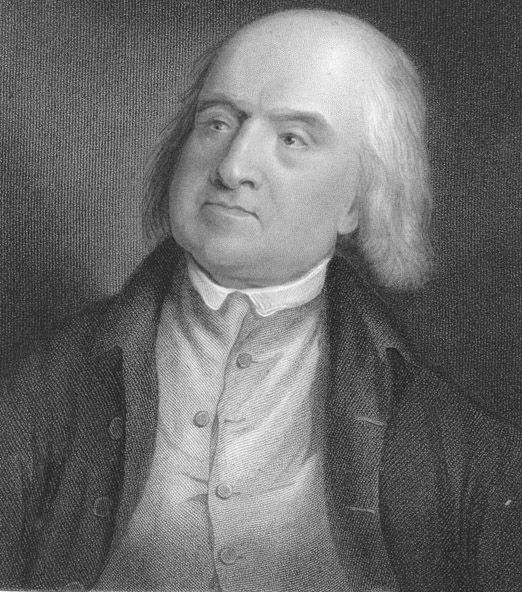
\includegraphics[width=50mm]{images/bentham.jpg}
  %     \caption{Jeremy Bentham}
  %   \end{center}
  % \end{wrapfigure}


\begin{quote}
\small Jeremy Bentham, The Rationale of Reward, Book 3, Chapter 1.からの抄訳。Peter Singer,
  Ethicsにも収録されている。江口聡訳.(c) EGUCHI Satoshi 2006。
\end{quote}

\vspace{2zw} 技芸(arts)と学術(sciences)を、全体として社会の幸福とのかかわりのなかで考察すると、これらは二つの部分に分けることができる。つまり、(1)娯楽(amusement)と好奇心(curiosity)のためのもの、(2)直接的・間接的な有用性のためのものである。人間の知識のこの二つの部門について、政府はまったく別の対処方法を必要とする。

娯楽ための技芸と学問ということで私が言おうとしているのは、ふつうは芸術(fine arts)と呼ばれているものである。たとえば、音楽、文学、絵画、彫刻、建築、造園などである。これらを枚挙することはここでは控えておくことになる。もし、このような枚挙を完全にするためにどうしても必要な形而上学的な議論に深く入りこんでしまえば、現在の論題からあまりにも離れてしまうだろうからである。あらゆる種類の娯楽がこの項目に含まれる。

(中略)

好奇心のための技芸と学術ということで私が言おうとしているのは、実際には快をもたらすが、それは芸術ほどではなく、また、一見したところ我々がそれが快を与えるということを否定したいと思うかもしれないようなものである。これは、これらの好奇心のための技術と知が、教養ある人々にとっては芸術ほどには快をを与えないというわけではない。しかし、これらの技術と知を研究しているひとびとの数の方は限られている。紋章学や純粋年代学(pure chronology){\――}現在は珍奇な言葉の寄せ集めしかもたらさない古代や外国の言語についての知識{\――}といった学問はこうした性質のものである。また古代の風習の研究なども、道徳性に対して応用することのできるなんからの教示や、なにか有益で望ましい知識をもたらさないのならば、この種の性質のものである。

これらすべての技芸と学術{\――}娯楽と好奇心のための技芸と学術の両方について語っているのだが{\――}が持つ価値は、それが生み出す快楽に正確に比例している。ある人々が技芸や学術に認めようと試みているその他の卓越性は、実はまったくのたわごとにすぎない。偏見を離れれば、押しピン遊びは音楽や文学といった技芸や学術と同じ価値がある。もしも押しピン遊びが、より多くの快楽を提供するとすれば、それはより多くの価値があることになろう。文学(poetry)や音楽はほんの少数の人々によってしか楽しまれない。押しピン遊びは常に無害である。同じことが文学についても常に主張できれば好都合だが、実際にはそうではない。実際のところ、文学と真理との間には、本性上の対立がある。それは文学の誤った教訓と虚構性である。文学者は常になにか偽であるものを必要としている。文学者が真理に土台を置くというふりをするときにも、その上にある装飾品はフィクションである。文学者の仕事はわれわれの感情を刺激し、偏見を助長することにある。真実、すなわちあらゆる種類の正確さは、文学者にとっては致命的である。文学者はなにごとも色眼鏡を通して見ねばならず、他の人々にも同じよう色眼鏡を通して見させようとするのである。たしかに、これまで高貴な魂(noble spirits)と呼ぶことのできる人々が存在しており、文学と哲学はともに彼らに多くを負ってきた。しかし、これらの例外は、この文学という魔術が生み出した不幸を償うものではない。もし文学と音楽が押しピン遊びよりも好まれるに値するとすれば、それは、まったく気むずかしい人々を満足させるよう計算されているからに違いない。

\section{快楽計算}
\begin{itemize}
\item 強さ、持続性、確実性、遠近性、多産性、純粋性、範囲が重要。
\item 快楽のリスト。
\end{itemize}

\fi

\section{ベンサムの功利主義}


\begin{itemize}
\item ベンサム、J.S.ミル。
\item 快楽と苦痛が重要。
\item 最大多数の最大幸福。関係者全員の快楽を最大にし、苦痛を最少にする行為・制度が正しい。
\item 各種の制裁をもちいて人々の行動をコントロールする。
\item 19世紀初頭のイギリス「哲学的急進派」の思想的基盤。19世紀後半にかけて、さまざまな社会改革運動に理論的基盤を提供。監獄の改革、婦人参政権を含む普通選挙、自由貿易、植民地制度改革、労働組合の合法化、公費による国民教育、言論出版の自由、秘密投票制、官吏任命制および業績主義、高利禁止法の廃止、地方政府の改革、海運の安全規定、衛生上の改革、公費による予防医療、統計の組織的蒐集、貧困者のための無料裁判、産児制限、煙害対策。
\item ミルの『自由論』。言論の自由と、個性の発展の尊重。
\end{itemize}


\begin{enumerate}
\item J. ベンサム(1748-1832)、J. S. ミル(1806-1873)など。

 \item 功利性の原理。いくつかの行動あるいは社会政策を選択する場合、関係者全員にとって最善の結果をもたらすものを選ばねばならない。「最大多数の最大幸福」。

   \begin{quote}\small{}

     「功利」または「最大幸福の原理」を道徳的行為の基礎として受けいれる信条にしたがえば、行為は、幸福を増す程度に比例して正しく、幸福の逆を生む程度に比例して誤っている。幸福とは快楽を、そして苦痛の不在を意味し、不幸とは苦痛を、そして快楽の喪失を意味する。この説がたてた道徳の標準について明確な意見を述べようとすれば、まだまだ多くのことをいわねばならない。とりわけ、苦痛と快楽の観念の中にどういうものが含まれるのか、どの程度までこれが未解決の問題として残されているかについて触れなければならない。しかし、こういう補足的な説明は、この道徳説がもとづいている人生観{\――}つまり、快楽、および苦痛の不在が、目的として望ましい唯一のものであるという人生観、さらに、ずべての望ましいもの〔それは功利主義においも他説同様たくさんある〕は、その中に含まれた快楽のために、または快楽を増し苦痛を防ぐ手段として、望ましいのだという人生観{\――}には影響を与えない。(ミル『功利主義論』第2章)

   \end{quote}

 \item 単純。平等(「誰もを一人として数え、誰も一人以上に数えない」)

 \item 各種のサンクション(制裁)を用いて、人々をコントロール。

 \item 19世紀初頭のイギリス「哲学的急進派」の思想的基盤。19世紀後半にかけて、さまざまな社会改革運動に理論的基盤を提供。監獄の改革、婦人参政権を含む普通選挙、自由貿易、植民地制度改革、労働組合の合法化、公費による国民教育、言論出版の自由、秘密投票制、官吏任命制および業績主義、高利禁止法の廃止、地方政府の改革、海運の安全規定、衛生上の改革、公費による予防医療、統計の組織的蒐集、貧困者のための無料裁判、産児制限、煙害対策。

\item 現在でも社会政策等に大きな影響。

\end{enumerate}


\section{トクヴィルのデモクラシー論}




\section{J. S. ミルのリベラリズム}

\begin{itemize}
\item 言論表現のほぼ絶対的自由の必要性。
\item (1) 政府批判のため、(2)真理の獲得のため、(3)批判検討のため。
\item 個性の擁護。幸福のためには自由な「生活の実験」による個性の発展が必要。
\end{itemize}

\if0

\begin{quotation} \small{}人類が、不完全であるかぎりは、さまざまな意見のあることが有益であるのと同じく、次のことが有益である。すなわち、さまざまな生活の実験があること、他人への危害がないかぎり自由な活動の場が多種多様な性格に対して与えられること。また、さまざまな生活様式をもし試みるのが適当と思う人があれば実際にやってみてその価値を明らかにすること、が有益である。要するに、第一義的に他人に関係しない事柄においては、個性が自己を主張することが、望ましい。その人自身の性格ではなくてほかの人々の幸福の主要な構成要素の一つであり、かつ個人的社会的進歩のまさに第一の構成要素をなすものが、欠けていることになるのである。・・・

  知覚、判断、識別感情、精神活動、倫理的好悪さえも含めた人間の諸能力は、選択という行為をする際にのみ訓練される。何事であれそうするのが習慣だからといってする人は、なんの選択もしない。彼は最善のものを見わけたり望んだりする練習ができない。肉体的能力と同じように精神的道徳的能力も、使われることによってのみ向上する。ただ、他の人々がするからするというのでは、これらの能力は少しも訓練されない。それはちょうどある事がらを、他の人々がそれを信じているという理由だけで信じるのど同様である。もしある意見の根拠が、その人自身の理性を納得させるものでなえければ、彼の理性はその意見を採用することによって強められはせず、むしろ弱められがちである。そして、行為への誘因が彼自身の感情や性格に一致しないようなものならば、〔愛情や他人の権利が関係していない場合〕それは彼の感情や性格を活発で精力的なものにするかわりに、不活発で鈍いものにするのに大いに役だつのみである。

  自己の生活設計を、自分のかわりに、世間や自分自身が属している世間の一部が選ぶのにまかせる人は、\ruby{猿}{さる}のような模倣能力のほかにはどんな能力も必要としない。自分自身で生活設計を選ぶ人は、彼のすべての能力を使用する。彼は、見る観察力、予測する推理力と判断力、決定に必要な資料を集める活動力、決定する識別力を使わなければならず、いったん決定をくだしたら、自己の熟慮した決定を守る確固とした意思と自制心を使わなければならない。そして、彼はこれらの能力を、自己の行為のうち、みずからの判断と感情にもとづいて決定する部分の大きさに比例して必要とし、また行使するのである。(J. S. ミル『自由論』)
\end{quotation}

\fi






\nocite{bentham1789:_introd_to_princ_of_moral_and_legis}
\nocite{bentham1825:_ration_of_rewar}


\ifx\mybook\undefined
\bibliographystyle{eguchi}  
\bibliography{bib}
\end{document} %----------------------------------------------------------------
\fi






%%% Local Variables:
%%% mode: japanese-latex
%%% TeX-master: t
%%% coding: utf-8
%%% End:

\ifx\mybook\undefined
\documentclass[uplatex,dvipdfmx]{jsarticle} \usepackage{mystyle}%\author{} %date{}
\title{ロマン主義、ヘーゲル主義、民族主義}
\if0 %----------------------------------------------------------------

\fi  %----------------------------------------------------------------
\begin{document}
\maketitle
\else\chapter{ロマン主義・ヘーゲル・民族主義}
\fi



\section{19世紀ロマン主義}

\begin{itemize}
\item 理性と普遍性を重視する啓蒙主義への反発。
\item 18世紀末から「ロマン主義」と呼ばれる思想・芸術運動が生じる。ドイツが中心。
\item 18世紀啓蒙主義の理性尊重への反発。ルソーらの人間的・自然的な感情を重視する立場からの影響。
\item ナポレオンの登場による英雄崇拝。
\item 芸術・宗教的感情の尊重。情熱的な恋愛の神聖視。
\item 文学ではゲーテ、シュレーゲル、ヘルダーリン、音楽ではベートーヴェンなどが主要人物。以降シューマン、ベルリオーズ、リスト、ワーグナーなど。
\item 個性、民族性、宗教的感情の重視。
\item 自然への注目。
\end{itemize}


\section{市民社会から国家主義へ}

\begin{itemize}
\item 18世紀末〜19世紀初頭にブルジョワ(有産階級)を中心にした「市民社会」がほぼ成立。資本主義。
\item 市民の政治的発言権。自由な競争。市民のなかでの貧富の差の拡大。
\item ホッブズ・ロック的な夜警国家から、より強力な権力をもった国家が求められるようになる。
\end{itemize}


\section{ナショナリズム}

フィヒテなど。





\section{ヘーゲル}

\begin{itemize}

\item ドイツからフランス革命を見たヘーゲル (1770--1831)は、人類の歴史を自由の実現する過程として捉えた。
個人はばらばらに存在するものではなく、具体的な社会制度(「人倫」)や組織のなかでこそ人間となる。

\item ヘーゲルの\emph{弁証法}という考え方は世界的に影響を与えた。
\item すべてのものは運動(変化)している。「正(テーゼ)」「反(アンチテーゼ)」の対立から「合(総合、ジンテーゼ)」が生み出される三段階を経てより高い段階に至る。

\item 歴史の発展も正・反・合の三段階を繰り返し、より大きな「自由」が実現される過程として理解できる。

\item \emph{人倫}の三段階。
  \begin{enumerate}
  \item \emph{家族}は自然的愛情に結ばれた共同体。男女\footnote{「男性は対外関係でたくましく活躍するもの、女性は受動的で主観的なもの」という対照がある。}の愛、その結果として子どもが生まれ、それは成長し独立した人格となって家族の外に出ていく。家族は共同体として存続するが、養育と教育によって子どもを自立させ、みずかから解体する。

\item \emph{市民社会}。独立したこどもは市民の一人として社会に参加する。市民社会は「欲望の体系」であり、各個人はみずからの欲望を追求するため労働に精をだす。しかし市民社会を成立させる市場の活動の結果、少数者への富の集中や多数者の窮乏化が起きる。

\item 中央集権化された\emph{国家}。個人の利益と全体の利益が一致。

  \end{enumerate}


% \section{ショーペンハウアー}


\subsection{発展する世界史}

\begin{itemize}
\item 歴史は一定の法則に従って発展しているという発想。
\item 古代は少数の人間のものだった自由が、次第に多くの人のものになってゆくという発展。
\item 「世界精神」。
\end{itemize}






\section{さらに学習するために}

宇野重規 (2013)『西洋政治思想史』、有斐閣。

ピーター・シンガー (1995)『ヘーゲル入門:精神の冒険』、島崎隆訳、青木書店。

\end{itemize}

\nocite{singer83:_hegel}

\ifx\mybook\undefined
\bibliographystyle{eguchi}
\bibliography{bib}
\end{document} %----------------------------------------------------------------
\fi






%%% Local Variables:
%%% mode: japanese-latex
%%% TeX-master: t
%%% coding: utf-8
%%% End:

\ifx\mybook\undefined
\documentclass[uplatex,dvipdfmx]{jsarticle} \usepackage{mystyle}%\author{} %date{}
\title{}
\if0 %----------------------------------------------------------------

\fi  %----------------------------------------------------------------
\begin{document}
\maketitle
\else\chapter{社会主義}\fi


\begin{itemize}

\item 18世紀末の都市化・工業化 → 貧富の差の拡大。
\item 資本主義の問題。貧富の差の拡大。
\item 資本家と労働者の階級対立。
\item オーエンの共産村。
\item サン・シモンの統制経済。
\item フーリエの理想的共同体の計画。
\item 平等の重視。 → 自由競争の否定、制限。生産手段の共有。
\item サン=シモンやフーリエ(仏)。 オーウェン(英)
\item → 小さな共同体での財産・生産手段の共有。

\end{itemize}


\section{初期社会主義}



\emph{ウィリアム・ゴドウィン} (1756-1836)『政治的正義』(1793)。無政府主義。富の平等な分配を要求。一夫一婦制の否定。


\emph{アンリ・ド・サンシモン}は貴族階級の出身だが、理想社会は貴族ではなく産業人(生産者)が政治的指導権を握るべきだと主張した。


\emph{シャルル・フーリエ}(1772-1837)は、各人の食欲や性欲といった本能的欲望の自由な充足が社会の目標であるとした。
そのため一夫一婦の結婚制度を否定する。400〜2000人程度の規模の共産村での生活を構想した。

成功した工場主である\emph{ロバート・オウエン}(1771-1848)は自分の工場で5歳の子供が1日13時間働いているのを見てショックを受ける。功利主義者ベンサムから影響を受け、児童労働を禁止するため工場法の成立のために尽力した。


『新社会論』。環境決定論。貧困層は道徳的にもあまりよくない状態にあるが、しかしこれは教育や環境の結果にすぎない。環境が労働者の資質を決定するので、労働者の生活・労働条件を決定する経営者に責任があると考えた。教育と環境を改善することによって性格形成・性格改善をめざす。また子どものための学校を工場に併設し、幼稚園の原型をつくった。


\begin{quotation}
子供にとって、子供の親にとって、社会にとってより良いことは、子供が12歳になり、教育を終え、要求される労働と作業に体が耐えられるようになるまで、労働を開始してはならないということである……。

人格の形成に関する国家計画は、どのような個人の立場にも関係なく、教育の近代的発展を含めなければならない。そして、帝国の国民であるすべての子供を除外してはならない。これを実現しないものは、排除すべき俯瞰用途不誠実の行動となり、社会における権利侵害となる……
% \footnote[p.247から孫引き。]{\citet{ishay04:_histor_human_right}}
。
\end{quotation}



\section{マルクス主義}

\begin{enumerate}

\item マルクス(1818--1883)
\item 資本主義社会批判。
\item 資本家階級と労働者階級の対立。
\item 労働者は労働力を\emph{搾取}されている。 → \emph{人間疎外}・労働疎外
\item \emph{唯物史観}。歴史は人類の経済活動の発展として見られる。生産力が向上すると従来の社会関係に矛盾が生じ、社会改革が必要になる。 → 歴史は階級闘争の歴史。
\item 共産主義の成立によって歴史は完成する。
\item 暴力革命も肯定。
\item → レーニン(1870--1924)。\emph{プロレタリアート独裁}。
\end{enumerate}

\subsection{ブルジョワ道徳批判}

\begin{itemize}
\item 既存の宗教、法律、道徳などは単なる歴史的・社会的立場に制約された「イデオロギー」。
\item 一般的な道徳は、ブルジョワ(中産)階級の利益になるよう構成されている。
\end{itemize}


\subsection{史的唯物論}

\begin{itemize}
\item 歴史は生産様式の変化によって区分される。
\item 生産力は歴史とととも増大する。
\item 社会革命は生産力の増大によって要求される生産関係の変化の反映。
\item 階級と階級闘争。
\end{itemize}




\subsection{共産主義}

\begin{quote}
  共産主義社会の高次の段階では、個人が分業に奴隷的に隷属することが消滅する。・・・労働が生活の手段であるだけでなく、生の第一の必要となる。個人の全面的発達とともに生産力も発達し、すべての協同的な富がいっそう豊かに溢れでるようになる。こうした後にはじめて、ブルジョワ的権利という狭い地平は踏み越えられ、社会は旗に書き込む{\――}各人からは能力に応じて、各人には必要に応じて!
\end{quote}


生産資源の共有。
「共産主義理論は一つのフレーズ、私有財産の廃止というフレーズに要約することができる」



\subsection{搾取}

\begin{itemize}
\item 資本家による労働力の\emph{搾取}が根本問題。搾取は他者の不公正な利用。
\item 資本家は労働者から、労働の対価として労働者に支払われる賃金以上の価値(剰余`価値)を生
  産物としてひきだす。
\item 労働だけが価値を創出するのであり、資本家は生産物の価値の一部をうけとる。またれゆえ労働者は創出した価値以下の価値しかうけとらない。それゆえ、労働者は資本家に搾取されている。
\item 労働者は生産財を所有しておらず、資本家のために働くよう\emph{強制}されている。

\item 「労働はあらゆる富の源泉である、と経済学者たちはいっている。しかし労働は無限になおそれ以上のものである。それは人間生活のいちばん根本の条件なのであり、しかもある意味では、労働が人間そのものを創造したといわねばならない。」

\end{itemize}

\subsection{疎外}

\begin{itemize}
\item 労働疎外。


\item 「労働はもっとも労働者自身のものでありながら、もっとも労働者が疎外されているものである」
\item 労働は人間のもっとも重要な能力。しかし賃労働によって、労働者の労働力はたんなる商品になり、資本家の統制のもとにおかれる。さらに、資本主義社会では労働者は労働において頭を使うことがなく、それゆえ本質的な満足を得られない。

  \begin{quote}
    労働者は、彼が富をより生産すればするほど、彼の生産力の力と範囲とが増大すればするほど、それだけますます貧しくなる。労働者は商品をよりおおくつくればつくるほど、それだけますます彼はより安価な商品となる。事物世界の価値増大にぴったり比例して、人間世界の価値低下がひどくなる。(『経済学・哲学草稿』)
  \end{quote}


\item 生産手段を共有することによって、労働者は自分の労働生活の編成方法について発言でき、本質的な満足を得ることが可能になる。

\end{itemize}



『ゴータ綱領批判』。能力に応じて働き、必要に応じて取る。



\section{プルードン}

「私的所有は盗みだ!」


\nocite{高晃公95:マルクス}
\nocite{大川正彦04:マルクス}
\nocite{kymlicka90:_contem_polit_philos}
\nocite{marx1848:_manif_kommun_partei:水田}
\nocite{marx1848:_commun_manif}


\section{修正社会主義、民主社会主義}

\begin{enumerate}
\item ベルンシュタインの修正社会主義。暴力革命を否定、議会主義による平和革命。

\item 民主社会主義。イギリスのフェビアン協会など。功利主義の影響。漸進的な社会改革による民主主義社会の実現を目指す。社会保障制度、産業資本の社会的管理、自由の保護。
\end{enumerate}


\ifx\mybook\undefined

\bibliographystyle{eguchi}
\bibliography{bib}


\end{document} %----------------------------------------------------------------
\fi




\section{マルクス主義}
\begin{itemize}
\item マルクスとエンゲルス(Friedrich Engels, 1830-1895)。
\end{itemize}

\subsection{ブルジョワ道徳批判}

\begin{itemize}
\item 既存の宗教、法律、道徳などは単なる歴史的・社会的立場に制約された「イデオロギー」。
\item 一般的な道徳は、ブルジョワ(中産)階級の利益になるよう構成されている。
\end{itemize}


\subsection{史的唯物論}

\begin{itemize}
\item 歴史は生産様式の変化によって区分される。
\item 生産力は歴史とととも増大する。
\item 社会革命は生産力の増大によって要求される生産関係の変化の反映。
\item 階級と階級闘争。
\end{itemize}




\subsection{搾取}

\begin{itemize}
\item 資本家による労働力の\emph{搾取}が根本問題。搾取は他者の不公正な利用。
\item 資本家は労働者から、労働の対価として労働者に支払われる賃金以上の価値(剰余`価値)を生
  産物としてひきだす。
  \item 労働だけが価値を創出するのであり、資本家は生産物の価値の一部をうけとる。またれゆえ労働者は創出した価値以下の価値しかうけとらない。それゆえ、労働者は資本家に搾取されている。
\item 労働者は生産財を所有しておらず、資本家のために働くよう\emph{強制}されている。

\item 「労働はあらゆる富の源泉である、と経済学者たちはいっている。しかし労働は無限になおそれ以上のものである。それは人間生活のいちばん根本の条件なのであり、しかもある意味では、労働が人間そのものを創造したといわねばならない。」

\end{itemize}

\section{疎外}

\begin{itemize}
\item 労働疎外。


\item 「労働はもっとも労働者自身のものでありながら、もっとも労働者が疎外されているものである」
\item 労働は人間のもっとも重要な能力。しかし賃労働によって、労働者の労働力はたんなる商品になり、資本家の統制のもとにおかれる。さらに、資本主義社会では労働者は労働において頭を使うことがなく、それゆえ本質的な満足を得られない。

  \begin{quote}
    労働者は、彼が富をより生産すればするほど、彼の生産力の力と範囲とが増大すればするほど、それだけますます貧しくなる。労働者は商品をよりおおくつくればつくるほど、それだけますます彼はより安価な商品となる。事物世界の価値増大にぴったり比例して、人間世界の価値低下がひどくなる。(『経済学・哲学草稿』)
  \end{quote}


\item 生産手段を共有することによって、労働者は自分の労働生活の編成方法について発言でき、本質的な満足を得ることが可能になる。

\end{itemize}

\subsection{共産主義}

\begin{quote}
  共産主義社会の高次の段階では、個人が分業に奴隷的に隷属することが消滅する。・・・労働が生活の手段であるだけでなく、生の第一の必要となる。個人の全面的発達とともに生産力も発達し、すべての協同的な富がいっそう豊かに溢れでるようになる。こうした後にはじめて、ブルジョワ的権利という狭い地平は踏み越えられ、社会は旗に書き込む{\――}各人からは能力に応じて、各人には必要に応じて!
\end{quote}

\begin{itemize}
\item 生産資源の共有。「共産主義理論は一つのフレーズ、私有財産の廃止というフレーズに要約することができる」
\item 暴力革命の必要性。
\item プロレタリア独裁。
\end{itemize}





\subsection{マルクス以後}

\begin{itemize}
\item 社会主義者の国際組織第一インターナショナル。(1866)
\item 無政府主義。バクーニンやクロポトキンなど。
\item 第二インターナショナル(1889)。
\item 暴力革命やプロレタリア独裁を否定する修正マルクス主義(ベルンシュタイン)→ 社会民主主義。穏健な改良主義。
\item 社会主義。フェビアン協会(1884)。社会改良、福祉厚生の向上。
\item ロシアでのソヴィエト革命(1917)。レーニン。
\item 毛沢東による中国共産党独裁(1949)。
\end{itemize}






%%% Local Variables:
%%% mode: japanese-latex
%%% TeX-master: t
%%% coding: utf-8
%%% End:

 \include{darwin2011}
\ifx\mybook\undefined
\documentclass[uplatex,dvipdfmx]{jsarticle}
\usepackage{okumacro,plext}
\usepackage{natbib}
\usepackage{url}
\usepackage{txfonts}
\usepackage[utf8]{inputenc}
\usepackage[T1]{fontenc}
\usepackage{otf}
%\usepackage{my_resume}
%\usepackage{graphicx,wrapfig}
%\usepackage[greek,english]{babel}
%\usepackage{teubner}
%\usepackage[dvipdfm,bookmarkstype=toc=true,pdfauthor={江口聡, EGUCHI Satoshi}, pdftitle={}, pdfsubject={},pdfkeywords={},bookmarks=false, bookmarksopen=false,colorlinks=true,urlcolor=blue,linkcolor=black,citecolor=black,linktocpage=true]{hyperref}
  \AtBeginDvi{\special{pdf:tounicode EUC-UCS2}}% platex-utf8 でも OK
\author{江口聡}
%\date{}
\title{19世紀の科学の発展}
\if0 %----------------------------------------------------------------

\fi  %----------------------------------------------------------------
\begin{document}
\maketitle
\else\chapter{19世紀の科学の発展}\fi



\label{cha:19}

19世紀は科学が開花した時代でもある。



\section{進化}



\subsection{ダーウィン以前}




\begin{enumerate}
 \item キリスト教的理解=「神が作った種」。デザイン論。時計を見れば時計職
       人がそれを作ったことがわかるように、生物のようによくデザインされたものを見ればそれを創造した者がいることがわかる。人間以外の生物は人間のために造られた。

\item 18世紀までの世界観。
\item デザイン論。人間も他の自然物も神がデザインした→動植物は人間が使
  う「ため」にある。
\item 存在の連鎖。大気→水→土→樹木→昆虫→爬虫類→魚類→両足獣→サル
  →人間
\item 生物の多様性。なぜこんなに多様な生物が存在するのか?
\item 博物学。
\item ビュフォン。
\item リンネ(1707--1778)の分類学。生物の世界に秩序を見つけようとする。


\end{enumerate}



\subsection{ダーウィンの進化論}

\begin{itemize}
\item ラマルク(1744--1829)の進化論。「生物はすべて前進する」。「獲得形質の遺伝」をもとにした用不用説。 ← 否定されてる。
\item ダーウィン(1809--1882)。ガラパゴス諸島の生物の多様性の観察。フィンチという小鳥の研究。
  フィンチの種類は多様で、その嘴は、その食べ物によって違う。ほんの少しの環境の違いに生物が適応している。園芸家の品種改良の観察。
\item 進化論の柱
  \begin{enumerate}
  \item 遺伝。子供は親の性質に似る。
  \item 変異。生物の個体には、同じ種に属していてもさまざまな変異が見られる。
  \item 「生存のための奮闘」(struggle for existence 生存競争、生存闘争)
  \item 自然淘汰(自然選択)。生物は多産で、生き残れるより多く生む。→ 競争。
  \item 変異のなかには、生存や繁殖に影響を与えるものがある。→有利な変異の保存。
  \end{enumerate}
\item 人間と動物の共通性。動物にも心や知性がある。
\end{itemize}




\subsection{よくある誤解}

\begin{enumerate}

 \item ×動物は種の保存のために生殖する
 \item ×低級な動物から高等な動物に進化してきた(→すべての生物は進化の結果)
 \item ×自然淘汰はなんらかの目的にむかっている(→淘汰そのものは無目的)
 \item ×進化は進歩である(→単なる変化にすぎない)
 \item ×人間はチンパンジーから進化してきた(→共通の祖先から進化してきた)

\end{enumerate}


\subsection{『人間の由来』}




\section{社会ダーウィン主義}

\begin{enumerate}
\item スペンサー(1820--1903)。万物は単純なものから複雑なものに進化する。
\item 最適者生存(survival of the fittest)。→ 弱肉強食、優勝劣敗 → 自由放任(レッセ・フェール)が最適な社会をつくる。

\item 社会進化論→ ナショナリズム。国家間、人種間、民族間の闘争を「進化論」から正当化。「適者生存」→欧米各国、特にナチス。→欧米の移民政策に影響。→ナチスドイツの民族浄化政策。

\item ← ハクスリー(1825--1895)は進化の法則に逆らうような倫理が必要と主張。
\begin{quote}
  治癒の見込みのない病人、老悴した者、虚弱な心身あるいは欠陥のある心身を有する者、過剰な新生児などは、ちょうど園芸家が欠陥のある植物や過剰な植物を間引きし飼育家が望ましくな家畜を屠殺するように、取り除かれることになろう。強くて健康な者、それもこの統治者の目的に最も適応するような子孫をつくるために注意深く縁組みされた者だけが一族を残すことを許されることになろう。(Th. ハクスリー)
\end{quote}

\end{enumerate}

\nocite{市野川容孝12:社会学}





\section{医学}



ゼンメルワイス。衛生。

パスツール。細菌の発見。

ナイチンゲール。統計学。


\section{精神医学}



フランスの精神医学者ピネル(1745--1826)。閉鎖病棟で鎖につながれている「狂人」を解放。病院の改善。

エミール・クレペリン(1856-1926)。精神医学の成立。精神病を早発性痴呆(統合失調症)と双極性障害(躁うつ病)に分類。

リヒャルト・クラフトエビング(1840-1902)。『性の病理学』。性的倒錯(変態性欲)の研究。

フロイト。ヒステリー症例の研究から「無意識」概念の提唱。「精神分析」という手法の開発。


\section{人体の測定、優生学}


ガルの骨相学。


\citet{darmon89:_medec_et_assas}

イタリアの医師ロンブローゾ(1836-1909)の「犯罪人類学」。『犯罪者論』犯罪者の身体を測定。生来性犯罪者の概念。
犯罪者は隔世遺伝(先祖返り)。
『天才論』。天才は生来性犯罪者や狂人と類似した特徴がある。
 → 人種差別的だと批判されるが、アイディアは現代の犯罪学にも影響。

 人体測定ブーム。
 \citet{darmon89:_medec_et_assas}




ダーウィンの従兄弟、フランシス・ゴルトン(1822--1911)。
統計学の基礎(回帰、相関など)。
指紋を統計的に処理し、犯罪捜査に使うことを提唱。
 人類遺伝学 → 優生学。人類の遺伝的改良。→ 各国に影響。




優生学的政策。
オーストラリア。1901年移民制限法。
米国。1907年断種法(インディアナ州)→30州。移民制限法 1924。白人と有色人種の混血を防ぐ。
ドイツ。1933年断種法。アルコール依存症患者、性犯罪者、精神障害者、遺伝病。
カナダ、ノルウェー、フィンランド、デンマーク、スイスetc.
マーガレット・サンガーらの産児制限運動とも関連。
日本でも第二次世界大戦前から各種の動き。戦後の優生保護法1948。
\citet{米本昌平00:優生学}など。


\section{科学・技術}



ワットの蒸気機関の発明 1769。スティーブンソンの蒸気機関車 1814。

1830年代に電信技術が実用化。1840年代にはモールス信号が一般化。

ファラデー(1791-1867)。電気分解、電磁誘導など。ベンゼン。イオン。

ボルタのボルタ電池。→ 電気めっき。

ノーベルのダイナマイト。→土木、戦争。

マクスウェル(1831-1879)。古典電磁気学の確立。電磁波(電波)の存在の予言。熱力学、統計学。
電磁波はヘルツによって発見される。 → マルコーニの無線電信 1895。

カール・ボッシュのアンモニア合成。→肥料革命。火薬の製造に必要な硝酸。



\section{心理学}



哲学 + 生理学 →
ヴィルヘルム・ヴントの実験心理学。1879年にライプチヒ大学に心理学実験室創設。
ウィリアム・ジェームズ。
20世紀初頭に学問分野として独立。
アルフレッド・ビネーの知能テスト。

\section{人類学}

生物学、地質学、地理学。
1857年、ネアンデルタール人の骨を発見。





\ifx\mybook\undefined

\bibliographystyle{eguchi}  
\bibliography{bib,library}


\end{document} %----------------------------------------------------------------
\fi






%%% Local Variables:
%%% mode: japanese-latex
%%% TeX-master: t
%%% coding: utf-8
%%% End:

 \include{19century}
\ifx\mybook\undefined
\documentclass[uplatex,dvipdfmx]{jsarticle}
\usepackage{okumacro,plext}
\usepackage{natbib}
\usepackage{url}
\usepackage{txfonts}
\usepackage[utf8]{inputenc}
\usepackage[T1]{fontenc}
\usepackage{otf}
%\usepackage{my_resume}
%\usepackage{graphicx,wrapfig}
%\usepackage[greek,english]{babel}
%\usepackage{teubner}
%\usepackage[dvipdfm,bookmarkstype=toc=true,pdfauthor={江口聡, EGUCHI Satoshi}, pdftitle={}, pdfsubject={},pdfkeywords={},bookmarks=false, bookmarksopen=false,colorlinks=true,urlcolor=blue,linkcolor=black,citecolor=black,linktocpage=true]{hyperref}
  \AtBeginDvi{\special{pdf:tounicode EUC-UCS2}}% platex-utf8 でも OK
\author{江口聡}
%\date{}
\title{19世紀の社会科学}
\if0 %----------------------------------------------------------------

\fi  %----------------------------------------------------------------
\begin{document}
\maketitle
\else\chapter{社会学の成立}\fi



\label{cha:19century}


\section{社会学の成立}

\section{コントの実証主義}

\begin{itemize}
\item コント (Auguste Comte, 1798--1857)。サン=シモンの弟子。
\item 人類の知的進歩。神学的段階(想像) → 形而上学的段階(理性・論理) → 実証的(科学的)段階 (観察、実証)。
\item 「社会学」。歴史学、心理学、経済学を統合。社会の秩序と人類の進歩に寄与する。
\end{itemize}



\section{社会学の成立}
\begin{itemize}
\item マルクス (Karl Marx, 1818-83)。『資本論』。宗教・思想・道徳などの上部構造は、経済という下部構造に依存する。
\item デュルケーム。(\'{E}mile Durkheim, 1858-1917)。『社会分業論』『宗教生活の原初形態』。『自殺論』。統計資料を駆使して、自殺を個人の心理ではなく社会的要因から説明。
\item ウェーバー(ヴェーバー)。(Max Weber, 1864-1920)。人間の内面から社会的行為を理解する理解社会学。『プロテスタンティズムの倫理と資本主義の精神』。資本主義の発展は、カルヴァン主義の禁欲と合理性。(⇔ マルクス)
\item ジンメル。(Georg Simmel, 1858-1918) 『貨幣の哲学』
\item 各種の統計の収集、分析 → 統計学の発展。エンゲルのエンゲル係数(家計における食費の割合)など。
\end{itemize}






\ifx\mybook\undefined
\bibliographystyle{eguchi}  
\bibliography{bib,library}


\end{document} %----------------------------------------------------------------
\fi






%%% Local Variables:
%%% mode: japanese-latex
%%% TeX-master: t
%%% coding: utf-8
%%% End:

\ifx\mybook\undefined
\documentclass[uplatex,dvipdfmx]{jsarticle}\usepackage{mystyle}
\author{江口聡}
%\date{}
\title{ナショナリズム、帝国主義、ファシズム、そして人権}
\if0 %----------------------------------------------------------------

\fi  %----------------------------------------------------------------
\begin{document}
\maketitle

\else\chapter{ナショナリズム、帝国主義、ファシズム、そして人権}\fi


\section{奴隷解放}

\begin{itemize}
\item  フランス 1784。
\item アメリカ。リンカーン。南北戦争。 1864。
\end{itemize}





\section{第一次世界大戦}

オーストリア・ハンガリー帝国が崩壊。


\section{ソビエト連邦の成立}

1917年ロシア2月革命、同年10月革命。1922年樹立宣言。一党独裁。レーニン死去後スターリンが独裁。ネップ(新経済政策)と呼ばれる計画経済。コルホーズなどでの農業集団化。


\section{ファシズム}
\begin{itemize}
\item 中間層を基盤とした大衆運動。
\item 反動。権威主義。

\item ナショナリズム。
\end{itemize}


\nocite{水田洋91:社会思想史への招待,山脇直司92:ヨーロッパ社会思想史,水田洋06:社会思想小史}


\subsection{国際連盟}

アメリカ参加せず。20年代なかばから30年代にかけて中米諸国が脱退、ソ連は1934年から。日本、ドイツ、イタリアが脱退。ソ連を除名。


\section{第二次世界大戦}


\section{国際連合}

1945年設立。


\section{人権宣言}

エレノア・ルーズベルトらが起草。








\section{さらに学習するために}

\begin{itemize}
\item エレノアの本。
\end{itemize}


\ifx\mybook\undefined
\bibliographystyle{eguchi}  
\bibliography{bib,library}

\end{document} %----------------------------------------------------------------

\fi





%%% Local Variables:
%%% mode: japanese-latex
%%% TeX-master: t
%%% coding: utf-8
%%% End:

\ifx\mybook\undefined
\documentclass[uplatex,dvipdfmx]{jsarticle} \usepackage{mystyle}%\author{} %date{}
\title{}
\if0 %----------------------------------------------------------------

\fi  %----------------------------------------------------------------
\begin{document}
\maketitle




\else\chapter{西洋思想の導入}\fi



\section{明治}


\subsection{福沢諭吉}

啓蒙思想家。『西洋事情』『文明論之概略』。『学問のすゝめ』。実学を推奨。スピーチとディスカッションの訓練の必要性を説く。

\subsection{中江兆民}

ルソーを紹介。『三酔人経綸問答』。

\subsection{立憲君主制}

大日本帝国憲法(明治憲法)。1889。伊藤博文らがドイツ憲法を手本に起草。天皇が元首。議会によらずに行使することのできる大権をもつ。


\subsection{貧富の差}

貧民の生活の紹介。

河上肇『貧乏物語』(1916)。

\subsection{産業化と労働者}

工場法、労働者運動。

\subsection{社会主義}

片山潜、幸徳秋水らが社会民主党を設立。
人類同胞主義、軍備全廃、階級全廃、土地・資本・交通機関の公有化、分配の公平、平等な参政権、教育の無償化。即日解散を命じられる。

1906年、日本社会党設立。議会主義と直接行動論が対立。






\section{大正デモクラシー}

民主化。

女性運動。



\section{ナショナリズム}

北一輝とか。

国粋主義。

京都学派。

\section{戦後}

新憲法。








\ifx\mybook\undefined
\bibliographystyle{eguchi}
\bibliography{bib}
\end{document} %----------------------------------------------------------------
\fi






%%% Local Variables:
%%% mode: japanese-latex
%%% TeX-master: t
%%% coding: utf-8
%%% End:

\ifx\mybook\undefined
\documentclass[dvipdfmx,uplatex]{jsarticle}
\usepackage{okumacro,plext}
\usepackage{natbib}
\usepackage{url}
\usepackage{txfonts}
\usepackage[utf8]{inputenc}
\usepackage[T1]{fontenc}
\usepackage{otf}
%\usepackage{my_resume}
%\usepackage{graphicx,wrapfig}
%\usepackage[greek,english]{babel}
%\usepackage{teubner}
%\usepackage[dvipdfm,bookmarkstype=toc=true,pdfauthor={江口聡, EGUCHI Satoshi}, pdftitle={}, pdfsubject={},pdfkeywords={},bookmarks=false, bookmarksopen=false,colorlinks=true,urlcolor=blue,linkcolor=black,citecolor=black,linktocpage=true]{hyperref}
  \AtBeginDvi{\special{pdf:tounicode EUC-UCS2}}% platex-utf8 でも OK
\author{江口聡}
%\date{}
\title{}
\if0 %----------------------------------------------------------------

\fi  %----------------------------------------------------------------
\begin{document}
\maketitle
\else\chapter{女性の解放}\fi

\section{第一波フェミニズム:女性参政権運動}


\subsection{欧米での女性運動}

欧米では、19世紀なかばに近代的な「人権」意識にもとづいて、女性の参政権や財産権、教育の機会などを求める女性運動が発生した。これらの運動は現在第一波フェミニズムと呼ばれる。

フランスでは、フランス革命勃発の後、フランス人権宣言(人および市民の権利宣言)(1789)(p. \pageref{french}参照)によって近代的「人権」が宣言される。宣言第一条では、すべての人が自由で権利において平等であること、第二条では政治的結合(国家や政府)の目的がひとの不可侵の権利の保全にあること、第三条ではすべての市民に法律の制定に参加する権利を認めた。しかしここで言われている政治形態に関する憲法審議のなかでは、選挙権をもつ者は能動市民(一定額の税金を納めている男子)に限られ、女性には選挙権も被選挙権も与えられていなかった。その他、ユダヤ人、有色の自由人、植民地の奴隷、奴婢等にも権利は認められなかった。1848年まで次第に権利を持つ者の範囲は拡大されたが、1848年にいたっても女性の権利は制限されていた。

米国では第一波の女性解放運動は奴隷制反対運動と強い結びつきがあった。1838年ニューヨーク州セネカフォールズでの女性権利大会大会の『女性の所信宣言』\footnote{p. \pageref{sentiment}参照}や、1856年オハイオ大会でのソジャーナ・トルースの演説(p.\pageref{truth}参)照が有名である。1865年、憲法修正第13条によって、奴隷制が廃止された。さらに憲法修正第14条で21歳以上の男性に投票権を認め、憲法修正第15条で人種、肌の色、以前の奴隷の身分等による差別を禁止した。しかし女性の投票権はいまだ認められなかった。1869年、全国婦人参政権協会(National Women's Suffrage Association, NWSA) や米国婦人参政権協会(American Women's Suffrage Association, AWSA)が結成された。男子普通選挙は1870年に施行されたが、男女ともに選挙権を持つ一般普通選挙は1920年になってから施行された。

一方英国では、女性運動は廃娼運動(売春禁止運動)と結びつきが強かった。1864年、性病の軍隊での性病の蔓延を防ぐための伝染病法(CD法)制定された。ジョセフィン・バトラーが売春婦のみを取り締り、買春者を取り締らないことは性道徳の\emph{二重基準(ダブルスタンダード)}であるとして伝染病法廃止を訴えた。同時に参政権運動も盛りあがりを見せ、1866年、J. S. ミルが婦人参政権を求める請願書を議会に提出したが、翌年の議会で否決された。英国で実際に男子普通選挙が行なわれるようになったのは1918年であり、一般普通選挙は1928年になってからであった。



% (マルクス主義。エンゲルス『家族・私有財産・国家の起源』。)

%  (フロイト)


\subsection{国内の女性運動}

それでは、日本国内では事情はどうだったろうか。

諸外国と同じように、国内でも女性運動は参政権運動の一部としてはじまった。明治民法のもとでは「家」制度が基本的だった。戸主(家長)が家族を統率し、戸主権と家産は長男子が継承する。また夫は夫婦の財産を管理し、子に対する親権をもつ。妻は無能力者とみなされ、妻には家督相続権がない。さらに妻には貞操義務があるが夫にはない、と男女は大きく不平等に扱われていた。

明治憲法(1889)で選挙権が与えられるのは、一定額を納税した男子だった。女性の政治活動は治安警察法第5条によって禁止された。1886年、キリスト教系の矯風会が社会風俗の改善を求め、未成年の禁煙、禁酒法の制定、売春の禁止(廃娼)などを求めた。

1911年、女性運動団体の青鞜社が結成される。1914年、機関誌『青鞜』で、貞操論争\footnote{生田花世が貧困から貞操を破ったことを告白。原田皐月は食べることより貞操を重んじるべきだと反論。平塚らいてうは男女の性道徳の歳を批判し、女だけに貞操を要求する道徳を否定。伊藤野枝は貞操観からの解放を提唱。} 堕胎論争\footnote{原田皐月が、「受胎したと云ふだけでは生命も人格も感じ得ません」として堕胎を肯定。伊藤野枝が母親の都合のために「いのち」を殺すことは自然を侮辱し「生命」を軽視した行為だと批判。平塚らいてうがさまざまな理由から堕胎もやむをえない場合があることを肯定。} 、廃娼論争\footnote{伊藤野枝が中上流の婦人団体の事業や活動の欺瞞を指摘し、特に矯風会の公娼廃止運動も批判。青山菊栄が野枝を批判し、公娼の悲惨な生活を指摘して公娼廃止が必要であることを主張。}、母性保護論争\footnote{与謝野晶子が、妊娠出産期の女性が国家から経済的な保護を受けることを要求することは、国家への寄食であり依頼主義であるとして批判。それに対して、平塚らいてうが母性保護を国家に求めるのは当然であると反論。山川菊栄が、この両者の立場は相反するものではなく、女性に二者択一を強いる経済関係そのものを改変しなければならないと主張。} など諸々の活発な論争が行なわれる\footnote{\citet{新フェミニズム批評の会98:青鞜を読む}を参照}。

1919年、新婦人協会が結成される。治安警察法の改正運動。1922年改正。妻の財産権、刑法の姦通罪削除、男女の機会均等などの要求。1924年婦人参政権獲得既成同盟会結成され、1925年、男子普通選挙が施行される(実施は1928年)。


戦後の新憲法と民法改正によって家制度は廃止され、公民権、参政権、教育の機会、法制上の妻の地位の平等が実現した。


\subsection{女性の政治参加への反対論と性差}

このように各国において、女性の政治参加には強い抵抗があった。ここで
その反対論の主なものを列挙してみよう。

\begin{itemize}

\item 男性の方がより有能である。「夫と妻とは、ただひとつの共通の関心をもっているとはいえ、その理解力も違っているので、時にはまた違った意志をもつのもやむをえまい。ところで最後の決定権すなわち支配権というものはどこかに置かれていなければならないので、自然それは、より有能で、より強い、男の方の手に置かれるのである。」(ジョン・ロック(1632-1704)『市民政府論』、岩波文庫, pp.84-85)

\item 女性は男性を助ける役目を果すことが自然である。「女性の教育はすべて男性に関連させて考えられなければならない。男性の気に入り、役に立ち、男性から愛され、尊敬され、男性が幼いときは育て、大きくなれば世話をやき、助言を与え、なぐさめ、生活を楽しく快いものにしてる、こういうことがあらゆる時代における女性の義務であり、女性の子どものときから教えられなければならないことだ」「男性は外、女性は内、これこそ自然の法則である」(ルソー(1712-1778)『エミール』下巻、岩波文庫p. 21)

\item 女性の本質は子どもを養育することにある。「女性の固有の特性は、子どもを教育することである。このようなことが家事に続く女性の任務であり、女性は生来的に徳を愛するように運命づけられているのである。(フランス保安委員のアマールの演説) (\citet{奥田暁子03:フェミニズム思想史}p. 73)

\item 女性は家事に向いている。「公務に従事できる市民は非常にわずかな数でしかないということは確かである・・・女性から家事を取りあげるとは、農民から鍬を、職人から仕事場を取りあげられないことと同様に、できないことである」(コンドルセ、\citet{奥田暁子03:フェミニズム思想史}, p.81)


\item 「女性には男性ほどの正義の感覚が見られない。」「好意や敵意の感情によって判断が左右されやすい。」(精神医学者 シーグムント・フロイト)

\item 女性には政治に必要とされる精神的・肉体的能力がない。
\item 女性の貞淑さや羞恥心が政治参加に向かない。
\item 女性は興奮しやすく錯乱・無秩序になりやすい。
\item 女性は家族の世話という仕事を捨てて政治に口を出すために家庭を出るべ
  きではない。

\end{itemize}
 
このように男女の性差が社会的な通念とされ、女性の政治参加の障害となると考えられたのである。


\subsection{J. S. ミルの『女性の解放』}


上のような女性の社会参加・政治参加に否定的な雰囲気のなかで、男女の平等を擁護する議論も多く提出された。フランス革命期に活躍したオランプ・ドゥ・グージュ(Olympe de Gouges, 1748-93)の『女性の権利宣言』(1791)やメアリ・ウルストンクラフト(Mary Wollstonecraft, 1759-97)の『女性の権利の擁護』(1791)などが有名であるが、最も洗練されており重要なものがイギリスの哲学者であり『自由論』の著者である J.  S. ミルの『女性の解放(\emph{Subjection of Women})』\citep{mill1869:_subjec_of_women}である。この著作は国内でも早くから翻訳され、女性運動に大きな影響を与えた。その議論は現在では当然視されることが多いものだが、基本的な知識としておさえておきたい。

\begin{itemize}
\item 女性の男性に対する法的隷属は誤りである。女性に平等な地位を認めることに対する反対は、議論の結果ではなく、実は\emph{感情}に根ざしている。女性の法的な従属は、それが人類にとって最良であるという理由によるものではなく、男性が強さにおいてまさっていうという肉体的事実が法律上の権利に変えられ、社会によって認められているにすぎない。女性がみずから進んで自分たちの無能力な状態を受けいれているという議論がある。しかし女らしくない望みは押えるようにという教育がなかったら、もっと多くの女性が抗議をするだろう。集団的に反抗することを女性が好まない理由のもう一つは、男性をひきつけるような人となることが女性の教育の最終目標になっているからである。

\item ひとは各々自分がもっとも好ましいと思う運命を試す自由を持つべきである。自由競争が行なわれれば、不適当なものは自然に排除される。法律上男女が平等であることは、家庭において道徳的情操を訓練するための方策としても有用である。政治生活や高報酬の仕事から女性をしめだすのは、家庭生活における女性の隷属を永久化するためである。ひとが各々そのもっとも好ましいと判断する運命を試す自由を持つことが近代社会の特色である。誰もたまたま自分の生まれついた運命に鎖で縛られている必要はない。したがって、女に生まれたからといって、その人が社会的な地位や職業につくことを禁じてはならない。もしその地位につくのに適切な女性を社会から排除すれば、それは実質的な損失となる。


\item 男性は支配し、女性は服従するのが天性であるという議論は無益である。両性の性質は現在の不自然な関係のなかで観察することしかできないからである。そのうえわれわれはどのような(社会や環境の)影響が人間の性格を形成するかについて無知である。

\item 男性は女性がどのような意見を持っているかを十分に知らないのだから、女性自身が語るべきことを語る自由を持たなければならない。
   

\item 女性の本性に自由な活動を許しても、女性がその本性に反して行動するということにはならない。自由競争の結果、女性は自分がもっとも必要とされ、最も適当である職務に従うようになるだろう。

 \item 女性を解放することにはさらに多くの社会的および個人的な利益がある。

   \begin{enumerate}
   \item 男性が根拠のない優越感を持ち尊大になることを防ぎ、
   \item 社会への奉仕に用いられる精神的活動を倍増させ、
   \item 男性とは違った視点からの意見の影響を増加させ、
   \item 各人の幸福の最も重要な要素としての自由を実現する、などである。
   \end{enumerate}

 \end{itemize}

 このようなミルの立場は、男女の性役割を認めたとしても、社会的効用および個人の幸福の観点からして女性に社会参加の自由を認める方がより好ましい結果をもたらす、という徹底して功利主義的でリベラルな立場である。そしてこの立場が、以降の女性解放の基本的な理論的支柱となった。


\section{第二波フェミニズム}



\subsection{大戦後}

第二次大戦後、日本を含め先進国では女性の参政権や法の前での男女平等は原則として実現された。しかしそれでも女性に対する実質的な差別の問題はなくならなかったと考える人びとがいた。


よく読まれたのが、\emph{シモーヌ・ド・ボーボワール Simone de Beauvoir}(1908-1986)の\emph{『第二の性』}(1949)である。「ひとは女に生まれない。女になるのだ。」「社会において人間の雌がとっている形態を定めているのは、生理的宿命、心理的宿命、経済的宿命のどれでもない、そうではなく、「文明全体」が「女」をつくりあげるのだ」と宣言し、自分自身や他の多くの女性の生の経験を詳細に検討した。女としての子ども時代からの成長、恋愛、性交渉、避妊、性病、妊娠、中絶、結婚、婚外交渉、売春など、それまで十分には議論されていなかった女性としてかかえる問題が赤裸裸に議論された。そして、男性中心的な思想や理論では理解することも解決することもできない「女の問題」が多数存在していることを指摘した。

%% 引用チェック


\emph{ベティー・フリーダン Betty Friedan}の(1921-)\emph{『女らしさの神話 Feminine Mystique』} (1963) (邦訳『新しい女性の創造』)は、戦後の豊かな米国中流階級の既婚女性を襲った満たされない心理状態を「名前のない問題」と名づけ分析した。女性が経済的に豊かになっても幸福を感じることができず、抑鬱状態にあるのはなぜだろうか、とフリーダンは問う。

\begin{quote}
  私は何がこんなに不満なんだろうと自分に問いかけます。私は健康だし、素晴しい子どもがいて、きれいな新築の家もあり、お金も十分持っている・・・とにかく、小さいころから、ずっと、誰か、それとも何かが、私の人生の面倒を見てくれていたような感じがします。——まず両親でしょう、それから大学に行って、恋愛をして、子どもができて、新しい家に引っ越すというふうに。そんな具合にいつも決まった目標があった。それである朝目が醒めてみると、これから先何を楽しみにすればいいのかわからなくなっていたのです。
\end{quote}

「名前のない問題」の原因は、女性の社会的自己実現欲求が阻害されていることにある。フリーダンは1966年全米女性機構(National Organization of Women, NOW)を結成し、リベラルな立場から女性差別の撤廃と女性の社会参画を目指した。彼女たちは、ミルに代表されるようなリベラリズムの立場をつらぬき、公的な領域への女性の社会進出をめざした。一方で家事や育児、性愛などの私的領域は基本的には個人の責任で解決すべき問題であるとした。

一方、19世紀後半からの自然科学の発展にともない、知性やその他の心理的特徴の生物学的・統計的分析が行なわれるようになった。男女の性差の科学的な研究がはじめられた。女性の知性の研究。骨相学や神経解剖学。女性と男性の脳には違いがある。女性は男性に比べて小さな脳を持ち、脳の大きさは知性をある程度反映していると考えられた。

% 1910年にはHelen Thompson Wooleyがそれまでの性差研究を批判。
%  1940年代、ビネーのIQ尺度調査での男女の性差研究。

% 「生まれか育ちか(nature vs nurture)?」

文化人類学の分野では、\emph{マーガレット・ミード}(Margaret Mead) (1901-1978)がが強い影響力を持っていた。ミードは南太平洋サモアのフィールドワークから、男性性や女性性が文化は社会によって多様であり、それぞれの社会はその社会特有のジェンダー秩序によって構造化されていると主張した\citep{ミード61:男性と女性}。たとえばサモアの人びとは西欧社会とは比べものにならないほど性的に自由であり、おだやかで対人関係での衝突が少なく、また西欧社会で思春期の少年少女たちが経験するような心理的葛藤を持たない。西欧社会の強い性規範は普遍的なものではなく、文化によって形づくられているにすぎない。ここから、文化決定論、文化相対主義と呼ばれる立場が有力になる。


性医学者\emph{ジョン・マネー}や精神科医\emph{ロバート・ストーラー} \citep{ストーラー73:性と性別}は、性転換者、衣裳倒錯者、生物学的に性に異常のある患者などを研究し、生物学的性別と社会的・文化的な性別は必ずしも一致しないと主張し、人間のジェンダー自認(gender identity)は生物学的要因ではなく、親の養育態度など心理学的要因によるものであるとした。ジェンダーはもともと西洋語の文法上の性の分類を示す用語である。たとえばドイツ語では太陽`die Sonne'は女性名詞であり、月`der Mond'は男性名詞である。いっぽう、フランス語で `le soleil' は男性名詞であり、月`la lune' は女性名詞である。このような名詞のジェンダー区分はしばしば言語的に恣意的・偶然的であり、それ以上の根拠を持たないことから、男女の性差に関しても生物学的な基盤を持たないものを「ジェンダー」と呼ぶようになったのである。そしてこのような「性差は養育の結果である」という観点は、女性解放運動に大きな影響を与えることになる。


\subsection{意識向上運動}

アメリカ公民権運動、あるいはフリーダンの著書や活動をきっかけにして、60年代末から、法や制度における男女平等だけでは女性の解放には十分ではなく、女性自身の意識改革が必要であるという自覚が生まれた。女性は、自分たちが内面化してしまっている「女らしさ」「男らしさ」などの規範意識や行動から逃れる必要があると考えられた。女性だけのグループを形成し、問題と直面した。このような運動は\emph{意識向上運動} (Consciousness Raising, CR)と呼ばれた。法や制度など公的な場での男女の不平等だけでなく、それまでは個人的 private な領域とされてきた家族や恋愛関係、性欲や性行動などが議論の題材として問題として扱われ、それまで個人的なものであるとされていた女性の種々の抑圧や差別の体験は、実は女性が共通してもつ社会的体験であることが「発見」された。「\emph{個人的なことは政治的である The personal is the political.}」という有名な宣言が第二波フェミニズムのモットーとなった。

これらのグループは、それまでのリベラルな女性平等運動に比して、女性差別を\emph{根本から}認識しつくがえそうとしてみずから「\emph{ラディカル}フェミニズム」を名乗った。


\subsection{男女関係の政治学}

ラディカルフェミニズムの中心人物の一人が、『性の政治学 (Sexual Polisics)』(1971) \citep{millett70:_sexual_politics}を著したケイト・ミレットである。ミレットによれば、ある人間のグループが他の人間のグループに支配される仕組が政治である。そして、\emph{家父長制(父権制、patriarchy)}とは、年長の男性が年少者を支配するに加えて、男性が女性を支配しているという年齢と性別による二重の制度である。家父長制はあらゆる政治的、社会的経済的形態にいきわたっており、恋愛関係や性関係なども例外ではない。

\begin{quotation}
  生得の権利によって統治する集団は、急速に消滅しつつあるが、にもかかわらず生まれによる一つの集団を、別の生まれによる集団が支配するという、古くからある普遍的図式が一つ残っている——性の分野にはびこっている図式がそれである。

  ・・・われわれの社会秩序の中で、ほとんど検討されることもなく、いや気づかれることさえなく(にもかかわらず制度化されて)まかりとおっているのが、生得権による優位であり、これによって男が女を支配しているのだ。この体制を通じて、「内部植民地化」がひどく巧妙なかたちで成しとげられてきた。・・・性による支配はわれわれの文化のおそらくもっともいきわたったイデオロギーとして通用し、またわれわれの文化のもっとも基本的な権力概念を与えている。

  これというのも、われわれの社会が、他のあらゆる歴史上の文明と同じく、父権制だからである。軍隊、産業、テクノロジー、大学、科学、行政官庁、経済——要するに、社会の中のあらゆる権力の通路は・・・すべて男性の手中にあることを思い起こせば、この事実はただちに明らかになる。(pp. 71-2)

\end{quotation}



このような「性の政治」は文化のあらゆる側面に染みわたっている。

男は攻撃的で知的で強く、女は受動的で感情的で無能で従順であるというステレオタイプ的視点が存在する。自然科学はそのようなステレオタイプ的視点を生得的なものとして正当化しようとする。しかし実際には「男らしさ」「女らしさ」は\emph{社会化の結果}でしなかない。

家父長制は女性を「妻」と「売春婦」、美醜、年齢といったさまざまな階級に分け、互いに敵対させる。また、男性は女性を経済的に支配している。

さらに家父長社会では、性と暴力が密接に結びつけられている。

\begin{quote}
  われわれは父権制と暴力とを結びつけて考えることには慣れていない。父権制は、暴力を使う必要はほとんどないほどに、その社会化の体制は完璧であり、その価値観にたいする一般の同意ぶりは徹底しており、人間社会に永年にわたって、あまねくいきわたってきたのだ。ふつうわれわれは過去の父権制の蛮行を、異国のあるいは「原始的な」習慣と考える。現在の蛮行は病理学的、ないしは例外的な行動に限られた、一般的重要性をもたない個人的逸脱的行為とみなされる。しかし、ほかの全体主義的イデオロギーと同様に(人種差別主義や植民地主義はこの点でいくらか父権制と類似している)、父権制社会における統制は、緊急事態にも、恒常的な威嚇の道具としても、暴力支配によらずしては完徹しないだろうし、操作不能にすら陥るだろう。
\end{quote}

このような暴力には、強姦、ポルノグラフィー、インドでの妻の殉死、旧中国の纏足、中絶の禁止がもたらす非合法の中絶、イスラムでの女性のベール、アフリカ諸国での性器切除(FGM)、人身売買、本人の意志によらない結婚、畜妾、売春などが含まれる。


宗教においても女性は常に劣位に置かれる。また処女性がさまざまな儀礼と禁令によって重んじられている。


\vspace{1zw}もう一人大きな影響力を持ったのが『性の弁証法』(1971) \citep{firestone70:_dialec_of_sex}を著したシュラミス・ファイアストーンである。彼女は一見望ましいとされるロマンチックな恋愛関係のなかにも男女の政治があることを指摘した。女性抑圧の根源は性の階級制度にある。男性は女性を恋愛と生殖を基盤として支配している。ファイアストーンは、「女と愛は、社会を支えている土台であり、このふたつを調べてみれば、文化の構造そのものを脅かすことになる」男性文化とは、見返りを求めない女の愛情の力に寄生したものであったし、いまもそうである。」という。

彼女によれば、男性優位の起源は、生物学的家族という生殖の基本単位にある。妊娠出産能力を持つ女性は生物学的家族に拘束され、社会は男女という不平等な生物学的階級に分断されている。一方、女性はセックスを武器に男性から感情的な安定や経済的な階級保障を引きだしている。

このような場で、「ロマンス」は「性による女性差別を強化する文化装置」として働いている。現在の社会では、女性は男性にとってただセックスの対象であり、女性は自分のことをエロティックな存在であると自認するほどになっている。その際、女性のセックスは規格品化されてしまっている。つまり女性は常に性的なものと考えられており、肉体的な属性によって自分の価値をはかるように強制されている。「女性の性の規格品化は、女性が、全体としての階級制に目隠しをされる過程であり、そのことは、男性の目には、女性は個性をもった個人としては見えないようになることを意味している」と言う。たとえば男性の「俺はブロンドが好きだ」という発言によってブロンドの女性は侮辱されたと感じる。それは自分を「他の女とは違ったものにしている肉体的な属性によって自分の価値をはかるようになっているからである。」

そしてファイアストーンは、このような性による階級支配を解体するには、(1)妊娠・出産・育児といった生物学的な専制からの女性の解放、(2)すべての人の経済的独立、(3)女性と子どものより広い社会との結合、(4)性の自由が必要であるとした。具体的には現在の閉鎖的な結婚家族制度を解体し、生活形態、性的志向などを自由に組み合わせたライフスタイルを選べるような社会が望ましいとした。



\subsection{性暴力}

第二波のフェミニズムは、理論的な側面だけでなく、
社会に浸透しているが隠されてしまっている性暴力に注目した。



\emph{スーザン・ブラウンミラー}の\emph{『われわれの意思に反して』} (邦訳『レイプ・踏みにじられた意思』) \citep{brownmiller75:_again_our_will} やスーザン・エストリッチの『リアル・レイプ』\citep{estrich87:_real_rape}は、「強姦とは無分別で抑えがたい欲望から生じる犯罪ではなく、征服欲にかられた者が相手を貶め、自分の物にするために行う敵対的で暴力的な行為である」として、性暴力が行なわれる現実の場を暴露した。ブラウンミラーは、強姦とは単に性欲に駆りたてられた男性が犯してしまう犯罪というだけでなく、「強姦とは、すべての男がすべての女を恐怖状態にとどめておくことによって成立する、意識的な威嚇のプロセスに他なららない。\citep[邦訳p.6]{brownmiller75:_again_our_will}」という。デートレイプ、ドメスティックバイオレンスなどそれまでは強姦と認められていなかった性暴力が暴露されることになった。



% 強姦は暴力かセックスか、男性は生物学的に強姦への傾向を持つか。

\emph{キャサリン・マッキノン}\citep{mackinnon79:_sexual_haras_of_workin_women} )は、セクシャルハラスメントを女性に対する差別であるとして批判し、法的な運動を起こした。マッキノンはまた、ポルノグラフィーをも批判する\citep{mackinnon93:_only_words}。「ポルノは理論、強姦は実践」であって、ポルノグラフィーは女性の従属と搾取を構造的に制度化し、強姦その他性暴力を促す。
% \emph{家父長制}(父権制、 partiarchy)。
% 暴力、男らしさの誇示、女性嫌悪、サディズム、同性愛恐怖、強姦、
% ポルノグラフィー。

買春に代表される\emph{性の商品化}は一夫一婦制と裏表の関係にあることが確認され、(1)女性の性を断片化し、「モノ」化する、(2)男性と女性の非対称性によって権力関係を強化し、(3)商品化に値する性とそうでない性とに女性の性を振りわけるとして強く非難された\footnote{ただし一方で、売春をセックスワークとして合法化するべきであるとするフェミニストも現われた。}。

このようにして、社会におけるさまざまな隠された性差別や性暴力の存在が、フェミニズムの批判的な眼差しのもとで次々と暴露され、問題化されていった。この分析の上で役に立ったのが、先に挙げた私的な関係での政治力学であり、また単なる生物学的な性差としてのセックスと、社会的に押しつけられたものとしてのジェンダーの区別だったのである。


\section{分散と反発}

\subsection{フェミニズムの分散}

しかし70年代からフェミニズムは急速に分散し多様化していった。ここでは詳しく見ることができないが、リベラル対ラディカルというフェミニズム内部での対立に加え、マルクス主義フェミニズム、精神分析派フェミニズム、ポストモダンフェミニズム、エコロジカルフェミニズム、ブラックフェミニズム、母性主義フェミニズム、カルチュラルフェミニズムとさまざまな「冠つき」フェミニズムが主張されるようになった。

% 現状では男女の真の平等は不可能であり、女性が真に解放されるためには\emph{強制的異性愛}に対抗し、女性同士での性愛による連帯が必要であると主張する人びとがいた。女性抑圧の根源は異性愛の強制であり、この異性愛の制度を崩壊させる必要がある。

% \begin{quote}
%   レズビアンとは何であろう。レズビアンとは、爆発点にまで達したすべての女性の怒りである。レズビアンとは、社会が女性に認める以上に、もっと全人的で自由な人間でありたいと願う、内なる衝動のままに行動する女性である。レズビアンとは、社会の最も基本的な役割である女性の役割に課せられた制限や抑圧を断固拒否した女性である。
% \end{quote}

なかでも、1984年に出版されたキャロル・ギリガンの『もうひとつの声\emph{ In a Different Voice}』\citep{gilligan82:_in_differ_voice}は大きな話題を読んだ。これは、道徳的思考の発達において女性と男性の間には大きな違いがあり、女性は、具体的な人間関係やケア(配慮)を重視して道徳的思考を行ない、男性の抽象的で、正義や権利を中心にした思考とは対照的であるとするものだった。



\subsection{進化論、社会生物学、遺伝学}


80年代後半から、生物学者たちが進化論や遺伝学、動物行動学の成果を踏まえて人間の「本性」について新しい見解を打ち出すようになった。われわれの性差はどの程度生物学・遺伝的的要因に由来するのか、どの程度が文化に左右されているのか?

先のキャロル・ギリガンに触発された心理学的・社会学的研究、\emph{エドワード・O・ウィルソン}らの1980年代から進化論を背景とした社会生物学が注目を浴びている。

また、先に挙げたマーガレット・ミードの研究は問題が多いことが指摘された。ミードはサモア島の恋愛と性愛はヨーロッパの基準に比して自由であり、また少年少女は思春期にヨーロッパの少年たちが体験する葛藤を経験しないと報告したが、これらは意図的に誤った情報を伝えられた結果であって、実際にはサモアでも強い性規範と思春期の葛藤が存在することが、デレク・フリーマン\citep{freeman83:_margar_mead_and_samoa}らによって確認された。

またストーラーの研究に反して、「文化的」であると思われていた性差はやはり生物学的な基盤を持つと主張されるようになっている。たとえば哲学者スティーブン・ピンカーはすでに確証された事実として以下のようなものを挙げる\citep{pinker02:_blank_slate}。

\begin{itemize}

\item すべての文化で、男性は女性より攻撃的で犯罪傾向がある。

\item 多くの性差は類人猿共通である。

\item 社会的条件づけが認められないような年齢の小児にも性差が認められる。また、女性として育てられた性器異常の男性の多くは、自分を男性と考える。したがって性自認は社会的条件づけの結果であるという説は疑わしい。

\item ミトコンドリアと細胞核のDNA比較調査から、ミトコンドリアの遺伝子の方が核より多様であることが発見された。男性の方が女性より繁殖成功率の幅が広い、つまり、残した子どもの数に個体間で大きな差があったことがうかがわれる。これは、男性の方がより乱交的行動傾向を持つことを意味するかもしれない。

\item 性ホルモンのレベルの違いに応じて攻撃性に変化があることが示されている。また、男女の脳には構造的な違いが存在する。女性は生理周期によって心的活動に影響を受ける。女性ホルモンが低濃度の時期は一般に男性の方が得意であるとされる分野(空間図形の回転など)のテストでで好成績をおさめる。

\end{itemize}

このような最近の研究は、先天的・生物学的な性差と社会的構築物であるジェンダーという単純な区分に対する疑いをひきおこしている。もっとも極端な社会生物学者のなかには、女性の社会進出を阻んでいるのは社会制度ではなく、むしろ女性自身が社会進出や昇進を望んでいないからであり問題はないとさえ主張する人びともいる。\citep{browne98:_david_labour}

\subsection{差異と平等、事実と価値、個人と集団}


ここまで、19世紀から20世紀にかけての女性解放運動を駆足で見てきた。

さて、最初の問いに戻ろう。「セックス」に加え、「ジェンダー」概念が必要とされたのはどうしてだろうか。上で見たような第二波フェミニズムが家父長制{\――}女性を抑圧する男性支配の権力制度{\――}を批判する動きのなかで、女性に対する抑圧を分析する手段として自然的・生物学的な性差であるセックスに加えて、たんに歴史的・偶然的に女性たちに押しつけられた性差としてのジェンダーが概念が必要とされたわけである。「ジェンダー」は女性に対する抑圧を分析する道具であった。

公的な場への女性の進出を求める古典的なリベラルな立場と、私的な局面こそ女性抑圧の場であるとするラディカルな立場、そしてその後のフェミニズムの分散とフェミニズムへの反発は、男女の差と男女の平等をめぐる争いであると言うことができる。自由か平等か、平等か差異か、性差はどの程度文化の影響を受けているのか、ということについては現在も議論が進行中である。

最後に二つの点について注意をうながしておかねばならない。

第一に、性差は集団としての平均的な差であり、個人の差ではないことである。生物学的な男女を比較すれば、平均した場合男性の方が身長が高いが、だからといってすべての男性が女性より背が高いわけではない。

第二に、より重要な点として、単なる事実に関する知識だけから、価値や規範を主張することはできない。「人間は病気になる」という事実から、「病気になってもよい」という価値に関する主張を導くことはできない。「セックス」の意味でも「ジェンダー」の意味でも、「性差」は事実に関する事柄であり、「平等」は実は「人々はその人に応じて平等に扱われるべきだ」という価値や規範にかかわる事柄である。

もちろん、集団としての男女の間にどのような差があるかという事実に関する問題は、よりよい社会を構想する上で非常に重要だが、それは性差の事実に関する知識から直接に導かれるわけではない。よりよい社会とはどのような社会であるかという価値にかかわる判断が必要なのである。



% 統計的に男女に性差があることはどういう意味を含むだろうか。
% 性差があることは女性差別とどうかかわるだろうか。最後に
% J. S. ミルの流れをひく現代の倫理学者ピーター・シンガーの
% 男女の平等に関する議論を簡単に見てみよう。

% シンガーの立場は伝統的なリベラルの立場であり、
% ラジカルフェミニストたちはおそらくこのような
% 形式的でリベラルな平等の原則によっては、女性に対する
% 差別は廃絶できないと主張するであろう。


\if0
\twocolumn{}
\section{資料}


\subsection{グージュ『女性の権利宣言』}


\subsection{ウルストンクラフト}



\subsection{女性の所信宣言 セネカ・フォールズ、1848年}
\label{sentiment}

  

人類の歴史の過程におき、それらのうちのある一部の人々が、従来占めていた地位と異なりはするが自然法と自然の神の法が彼らに授けた地位を、世界の人々のなかで占めなければならなくなった時に、人類が行ってきた意見表明に対して当然の敬意を払おうとするならば、なぜ自分たちがそのような道程を取らざるを得なくなったかという理由をその人々は宣言すべきである。

よって、わたしたちは、以下の真実を自明の理として宣言する。すべての男性とすべての女性は平等に造られていることを、彼らはともに造物主によって一定の不可譲の諸権利を賦与されていることを、これらの諸権利のなかには、生命、自由、幸福の追求の権利が含まれていることを、これらの諸権利を保障するために政府は創設され、その正当な権力は被治者の同意に由来することを。これらの目的に害をなす政府があるならば、その政府に対する忠誠を拒否し新しい政府の創設を主張することは、その政府に忍従を余儀なくされている人々の権利である。新しい政府は、彼らの安全と幸福にもっとも効果があると思われる諸原則に基礎を置き、そのような形体へと政府の権限を組織するものでなければならない。たしかに、長く存続した政府が軽微で一時的な事由で変更を受けるべきではないことは、分別の命じるところではあるのだが、その結果のすべての経験が示すところは、人間には、自分たちが慣れ親しんできた形体を廃止してあるべき状態に戻るよりは、害悪に耐えうる間はこれに耐える傾向がある、ということである。しかしながら、常に同じ目的を果たすための長期にわたる一連の権力の濫用と簒奪が、人々に絶対的な専制を強いようとする意図を明らかにする場合には、その政府を捨て去り自らの将来の安全のために新しい防護の組織を備えることこそが、人間の義務である。そして、現在の政府のもとで女性たちが耐えてきた忍従こそ、まさにそのような忍従だったのであり、また、本来その資格がある平等な地位を女性たちが今この時要求せざるを得ないのは、まさにそのようなやむにやまれぬ必要性からなのである。

人類の歴史は、女性に対する男性の絶対的な専制の確立を直接の目的とした、男性による女性に対しての権利侵害と剥奪の繰り返しの歴史である。これを証明するために、公平なる世界に向けて、以下の事実を明らかにしよう。

男性は、不可譲の権利である選挙権の行使を、決して女性に認めてこなかった。

男性は、女性がその制定過程に何の発言権も持っていない法に、女性を従わしめようとしてきた。

男性は、もっとも無知で身分が低い男性であろうとも、自国民であるか外国人であるかを問わず与えられている諸権利を、女性には制限してきた。

男性は、選挙権という市民として第一の権利を女性から奪い、それによって立法府で女性が代表されないままにしておくことによって、女性をあらゆる面から抑圧してきた。

男性は、女性が結婚した場合には、法律的に民事上の無能力者としてきた。

男性は、女性が自ら働いて得た賃金をも含むあらゆる財産上の権利を、女性から奪ってきた。

男性は、多くの犯罪を、夫の面前で行われたならば妻がそれらの罪を犯しても不可罰にすることで、女性を道徳的に責任を取れない存在にしてきた。法が妻の自由を奪い貞操を管理する権限を夫に与えたせいで、婚姻契約において妻は夫への恭順を約束することを余儀なくされ、夫は事実上、妻の主人となっているのである。

男性は、離婚法を制定するに際し、何が離婚の正当な事由となるかについて、また別離の場合に誰に子供の監護権が与えるかについて、女性の幸福には一顧だにしなかった。離婚法は、すべての場合において、男性の優位という誤った前提に立っており、男性の手にすべての権力を委ねているのである。

男性は、既婚女性としてのすべての権利を女性から奪っただけでなく、女性が独身で不動産を所有する場合には、税を課して政府を支えさせるが、政府がこの女性の存在を認めるのは、彼女の財産が政府にとって利益を生じるときのみである。

男性は、利益のある仕事のほとんどすべてを独占してきたのであり、女性が就くのを許された仕事からは、女性はほんのわずかの報酬しか得られない。男性は、女性に対し、男性によって最も名誉あると思われる冨と特典へのあらゆる道を閉ざしている。名を知られた神学、医学、法学の教師は、女性にはひとりもいない。

男性は、女性が十分な教育を受ける機会をなくしてきた。あらゆる大学教育は、女性に門を閉ざしている。

男性は、使徒伝の権威を理由に、いくつかの例外はあるが教会の職務への公的な参加から女性を排除したり聖職から女性を排除することによって、国家において従属的地位しか与えなかったのと同じように教会においても従属的な地位しか、女性に与えてこなかった。

男性は、男女で異なる道徳律を世の中に示すことにより、人々に誤った道徳観を創り出した。この道徳律へに違反すれば、女性は社会から締め出されるが、男性の場合は、許容されるだけでなくほとんど問題にされない。

男性は、女性の行動範囲を定め得るのはその女性の良心と彼女の信じる神のみであるにもかかわらず、これを自分たち男性の権利であると主張して、エホバその人の特権を奪い取ってきた。

男性は、為しうるかぎりのあらゆる方法でもって、自分たちの力についての女性の自信を砕き、女性の自尊心を弱め、女性が従属的で屈辱的な人生に甘んじるように努めてきた。
  

さて、この国の半分の人々が選挙権を完全に奪われ、社会的にも宗教的にも劣位におとしめられていることを考慮し、また上記のような不正な諸法を考慮し、さらに、女性たちが、虐げられ抑圧され自分たちの最も神聖な諸権利を不正に奪われていると感じているがゆえに、わたしたちは、合衆国市民として女性に属するすべての権利と特権が、直ちに女性たちに認められるべきであると主張する。
  
わたしたちの目の前にある偉大な事業を始めるにあたり、かなりの誤解や間違った理解、嘲笑を受けるだろうことを予想している。しかし、わたしたちは、自分たちの目的を達成するために、できる範囲のすべての手段を利用するつもりである。わたしたちは、職員を雇い、パンフレットを配布し、州と連邦の立法府に請願し、聖職者と出版界に私たちへの協力を要請するよう努める。わたしたちは、この会議に続き、この国の各地で次々と同じような会議が続かんことを希求する。


\subsubsection*{決議}





(以上に鑑み、)自然の偉大なる教えが、「人間はその人自身の真の実質的(substantial)幸福を求める」ということであることは、広く知られている。ブラックストーンは著書の「法律釈義」のなかで、この自然法は、人類と同じくらい古く、神ご自身が命じたものであって、当然あらゆる義務に優越する、と述べている。自然法は、世界中で、あらゆる国々で、あらゆる時代において、人々を拘束する。人間の法の中でこの法に背く法は、何の効力も持たず、一方、効力のある法は、その力のすべて、その効力のすべて、その権威のすべてが、直接的にも間接的にも、本来の法であるこの自然法に由来するのである。ゆえに、わたしたちは、以下のことがらを決議する。
  
自然の教えこそが「あらゆる義務に優越する」がゆえに、いかなる形であれ女性の真なる実質的幸福に相反するような法は、自然の偉大なる教えと矛盾するものであることを、決議する。

自分たちの良心にかなった社会的地位を女性が占めるのを阻んだり、男性の地位よりも劣った地位に女性を位置づけたりするあらゆる法は、偉大なる自然の教えに反しており、ゆえに何の力も権威も持たないことを、決議する。

女性は男性と対等であり、造物主によってそのように作られており、人類の至高の徳に従うならば女性はそのようなものとして認められるべきことを、決議する。

この国の女性たちが、彼女らがそのもとに生きる法について知識を得るべきこと、また彼女らが、現在の自分の地位で満足だと宣言することで自分たちの卑しい地位を明らかにしてしまったり、自分が望んでいる権利はすべて手にしていると主張して無知をさらけだしたりすることがないようにと、決議する。

男性が自分たちの知的優越性を主張する一方で女性に道徳的優越性を与えていることに鑑みれば、あらゆる宗教的な会合において機会がある場合には、女性が演説し説教するように推奨することは、まったくもって男性の義務であることを、決議する。

社会において女性に求められるのと同じだけの貞淑さ、繊細さ、洗練が、男性にも求められなければならず、これを破った場合には、男性にも女性にも同じだけの厳しさで対応がなされねばならないことを、決議する。

女性が聴衆に向けて話しかけたときにしばしば投げかけられる不躾で不作法な非難の声は、女性を力づけようという気持ちでステージ、コンサート、サーカスでの女性の演技や発表を見に来ている人たちからは、生じるべくもないものであることを、決議する。

聖書の歪曲した適用によって生じたものであり、市民の心を腐敗させてしまう厳しい制約に対して、女性はあまりにも長い間不満を覚えずにいたのであるが、今や、偉大な造物主が彼女に課したより大きな領域へと動かねばならないときが来たことを、決議する。

選挙権という女性の神聖な権利を確実に手にすることが、この国の女性たちの義務であることを、決議する。

  人権の平等は、人間が持つ能力と責任が[性にかかわらず]同じものであるという事実から、必然的に帰結するものであることを、決議する。

  ゆえに、以下を決議する。造物主によって自分たちの行為に関して[男性と]同一の能力と同一の責任を与えられているのであるから、あらゆる正当な手段によってあらゆる正当な主義主張を訴えていくことが、男性同様女性の権利であり義務であることは明らかである。とりわけ、道徳と宗教という重要な課題に関しては、私的生活においても公の場においても、利用に問題のないあらゆる手段を利用し、開催に問題のないあらゆる集会で、文章を書いたり公演したりすることで、男性の同胞とともにこれらの課題にかんして啓蒙を行うことに参加するのが、女性の権利であることは自明である。そして、これらのことは、神に教えられた人間の本性の諸原則から生じた自明の真理であり、これらに反するどのような習慣や権威も、近代のものであれ恐ろしい制裁を伴う古代のものであれ、自明の誤りとみなされ、人類の存在とあい争うものなのである。

  [最後の会合で、ルクレシア・モットは、次の決議を提案し取り上げた。]

われわれの主張が迅速に達成されるためには、聖職の独占の打倒を求めての、また、さまざまな交易、専門職、商業に対し、男性と平等な参加を女性に保障することを求めての、両性によるところの熱心でたゆまぬ努力が必要であることを、決議する。
\begin{flushright}
  (澤敬子訳)
\end{flushright}





\subsection{ソジャーナ・トルースの演説}
\label{truth}
「白人男性はやがて権利について話し合っている南部の黒人と北部の女性の間で板挟みになるだろう。しかしここで一体何について話しあっているのかい。あの向うにいる男性は、女が馬車に乗るのに手を貸したり、抱き上げて溝を渡したり、いたるところで一番いい場所を譲る必要があると言っている。今までだれも私を馬車に助け上げてくれたり、田圃から引っ張り上げてくれたり、最上の場所をくれたりはしなかった。私は女じゃないのかい。見てご覧、私の腕を・・・土を耕し、苗を植え、収穫を納屋へ運んで働いてきた。男だって私には勝てない。それでも私は女ではないのかい。私は男と同じくらい働き、男と同じくらい食べることができる。そして同様に苦痛に耐えることができる。だからって、私は女ではないのかい。私は13人の子どもを生み、みんな奴隷に売られていった。泣き叫んでもイエス様以外だれも私の叫びを聞いてくれなかった。それでも私は女ではないのかい。

そこの黒い服を来た小さな男の牧師は男と同じ権利を持つことはできない、なぜならキリストは女ではなかったから、と云う。キリストはどこからきたんだい。・・・神様から、そして女から生まれたのだ。男は神とはなんの関係もなかった。(後略)」

\begin{flushright}
  (奥田暁子訳)
\end{flushright}


\section{さらに学習するために}

\begin{itemize}
\item 辻村みよ子、『女性と人権』、日本評論社、1997。
\end{itemize}


\fi
\ifx\mybook\undefined
\bibliographystyle{eguchi}  
\bibliography{bib,library}
\end{document} %----------------------------------------------------------------
\fi






%%% Local Variables:
%%% mode: japanese-latex
%%% TeX-master: t
%%% coding: utf-8
%%% End:


\chapter{現代の議論}

\section{ハイエク}


\section{バーリン}






\section{福祉リベラリズム}


\subsection{公正としての正義}
\begin{itemize}
\item ジョン・ロールズの『正義論』(1971)
\item 人間にとってなにが「善」であるかは公共的な立場からは解決不可能。→ なにが当人にとって
「善」であるかは当人の判断にまかさられねばならない。

\item 法や社会制度を考える上では「善」ではなく「正しさ」を問題にするべき。
(「善」に対する「正」の優位)
\item 正義こそが社会制度の第一の徳目。
\item 社会とは各人がそれぞれの善を追求する「相互利益を求める協働事業」。
\item 利害の不一致がある状況で、社会的な便益を適性に分配するにはどうしたらよいか?原理が必要。
\item 自由で平等な個人からなる「原初状態」を仮想してみる。各人は合理的だが、自分自身の属性を知らないと仮定(無知のヴェール)。
\item 無知のヴェール。自分の現実の社会的階層、社会的地位、性別、資産、精神的・肉体的能力を
  知らないとする。
\end{itemize}

\subsection{正義の二原理}

\begin{itemize}

  \item 各人は、すべての人びとにとっての同様な自由な体系と両立しうる最大限の自由への平等な権利を持たなければならない。
  \item 社会的・経済的不平等は、次の二つの条件を満たすように配置されなければならない。
\begin{enumerate}
    \item 最も恵まれない人びとの最大限の利益となるように
    \item 公正な機会の均等という条件の下ですべての人に開かれた職務や地位にのみともなうように。
    \end{enumerate}

  \begin{quote}
    福祉国家的資本主義は、財産や技能の当初の分配を所与の実質的な不平等として容認し、その上
    で事後的に所得を再配分しようとする。これにたいして財産所有の民主主義は、財産や技能の当
    初の分配における平等を求めるが、所得の再配分措置にたいしては、それほど重きをおかない。
  \end{quote}

\item 功利主義者は所有権に二次的な価値しか認めない。あくまで効用(人びとの幸福)の最大化が目標。

\end{itemize}


\section{リバタリアニズム(自由優先主義)}

\begin{itemize}

\item ロバート・ノージックの『アナーキー・国家・ユートピア』(1974)
\item ノージックのような自由優先主義(リバタリアン)によれば、暴力や詐欺のような不正な手段
  によらずに、正当に獲得した財産であれば、自由に使ってもよいとされる。私的所有権はほぼ絶
  対。
  \item 人びとは自分自身を所有する。
  \item 世界は原初的には誰のものでもない。
  \item 世界にはたらきかけ、自分自身の労働によって獲得したものはその人のものである。
  \item 他者の状態を悪くしないかぎり、世界の均等ではない取り分にたいする絶対的権利の獲得が可能である。
%   \item 世界の均等ではない取り分にたいする絶対的権利の獲得は比較的容易である。
   \item 一度、人びとが私有財産を占有すれば、資本や労働の自由市場が道徳的に要請される。

   

\end{itemize}


\section{共同体主義}




\nocite{nozick74:_anarc_state_and_utopia}
\nocite{有福孝岳99:エチカ,坂井明宏07:現代倫理学}
\nocite{rawls71:_theor_of_justic}
\nocite{川本隆史95:現代倫理学の冒険}




% \appendix{}
% 
\chapter{思想史簡易年表}



\bibliographystyle{jecon}  
\bibliography{bib}

\end{document} %----------------------------------------------------------------







%%% Local Variables:
%%% mode: japanese-latex
%%% TeX-master: t
%%% coding: utf-8
%%% End:
